\documentclass{article}


% if you need to pass options to natbib, use, e.g.:
%     \PassOptionsToPackage{numbers, compress}{natbib}
% before loading neurips_2024

% ready for submission
\usepackage{neurips_2024}


% to compile a preprint version, e.g., for submission to arXiv, add add the
% [preprint] option:
%     \usepackage[preprint]{neurips_2024}


% to compile a camera-ready version, add the [final] option, e.g.:
%     \usepackage[final]{neurips_2024}


% to avoid loading the natbib package, add option nonatbib:
%    \usepackage[nonatbib]{neurips_2024}


\usepackage[utf8]{inputenc} % allow utf-8 input
\usepackage[T1]{fontenc}    % use 8-bit T1 fonts
\usepackage{hyperref}       % hyperlinks
\usepackage{url}            % simple URL typesetting
\usepackage{booktabs}       % professional-quality tables
\usepackage{amsfonts}       % blackboard math symbols
\usepackage{nicefrac}       % compact symbols for 1/2, etc.
\usepackage{microtype}      % microtypography
\usepackage{xcolor}         % colors

\usepackage{amsmath} 		% maths
\usepackage{graphicx}		% figures
\usepackage{amsthm}			% proofs
\usepackage{multirow}


\title{SATURN: Splitting Approach on Tensorized Ubiquitous Regression Networks}


% The \author macro works with any number of authors. There are two commands
% used to separate the names and addresses of multiple authors: \And and \AND.
%
% Using \And between authors leaves it to LaTeX to determine where to break the
% lines. Using \AND forces a line break at that point. So, if LaTeX puts 3 of 4
% authors names on the first line, and the last on the second line, try using
% \AND instead of \And before the third author name.


\author{%
	A.~M.~Kharazi\\
	Department of Computer Science\\
	Tarbiat Modares University\\
	Tehran \\
	\texttt{am.kharazi@modares.ac.ir} \\
	\And
	M.~Badzohreh\\
	Department of Computer Science\\
	Tarbiat Modares University\\
	Tehran \\
	\texttt{noemail} \\ %%TODO
	\And
	M.~Rezghi\\
	Department of Computer Science\\
	Tarbiat Modares University\\
	Tehran \\
	\texttt{noemail} \\ %%TODO	
%  David S.~Hippocampus\thanks{Use footnote for providing further information
%    about author (webpage, alternative address)---\emph{not} for acknowledging
%    funding agencies.} \\
%  Department of Computer Science\\
%  Cranberry-Lemon University\\
%  Pittsburgh, PA 15213 \\
%  \texttt{hippo@cs.cranberry-lemon.edu} \\
  % examples of more authors
  % \And
  % Coauthor \\
  % Affiliation \\
  % Address \\
  % \texttt{email} \\
  % \AND
  % Coauthor \\
  % Affiliation \\
  % Address \\
  % \texttt{email} \\
  % \And
  % Coauthor \\
  % Affiliation \\
  % Address \\
  % \texttt{email} \\
  % \And
  % Coauthor \\
  % Affiliation \\
  % Address \\
  % \texttt{email} \\
}


\begin{document}


\maketitle


\begin{abstract}
%  The abstract paragraph should be indented \nicefrac{1}{2}~inch (3~picas) on
%  both the left- and right-hand margins. Use 10~point type, with a vertical
%  spacing (leading) of 11~points.  The word \textbf{Abstract} must be centered,
%  bold, and in point size 12. Two line spaces precede the abstract. The abstract
%  must be limited to one paragraph.
Convolutional Neural Networks often contain fully connected layers after their convolution phase, which requires the data to be flattened. Despite empirical success, this flattening ruins the multidimensional structure of the input data and increases the number of parameters, which may cause overfitting. Given the tensor nature of the input data, fully connected layers can be replaced with tensorized low-rank layers, which, besides considering the nature of the data, reduce the number of parameters. However, these layers perform poorly when the approximated rank is too low. To address this issue and further reduce the number of parameters while preserving the quality of the network, we propose a framework that, by using two splitting methods, transforms the multidimensional tensor into a thinner and higher-order tensor and applies tensorized layers on this high-order tensor. This leads to fewer parameters and less computational cost while preserving the quality of the network. In our experiments, evaluated on CIFAR10, MNIST, and Tiny ImageNet-200, we have successfully reduced the classifier parameters of well-known models such as VGG19, ResNet50, and ResNet101 by more than 95\%, while also achieving better accuracy and overcoming overfitting. Compared to traditional state-of-the-art models, our approach achieves significant parameter reduction and compression while preserving accuracy.
   
\end{abstract}


%\section{Submission of papers to NeurIPS 2024}
\section{Introduction}
\label{sec:introduction}
Convolutional networks are one of the most important architectures in deep learning, forming the basis for machine vision applications \cite{r35}. The most important point in the efficient architectures of convolutional networks is their high number of layers and, naturally, their large number of parameters, which, in addition to requiring a large amount of data for learning, makes it impossible to use these architectures even in the testing phase on medium or weak processing devices. Therefore, in recent years, many efforts have been made to reduce the number of parameters while maintaining the quality of these networks \cite{r1,r2,r3,r4}. Convolutional networks consist of two main parts: the convolutional layers for feature extraction followed by the MLP layers. Both of these parts play a role in increasing the number of parameters. In recent years, various efforts have been made for the convolutional part. Some methods, after training, aim to reduce the number of parameters and approximate the network for the testing part \cite{r36}. However, some approaches initially aim to replace the network layers with lighter layers, which in recent years, the second approach has received more attention due to its practicality \cite{r32}. Since in each convolutional layer, the input and output channels and the parameters are tensors, the use of tensor approximations has a better match with the network structure, and in both of the approaches mentioned above, it is one of the most common and effective methods in this field.

On the other hand, every convolutional neural network ultimately ends with MLP layers for classification. Therefore, in this phase, the three-dimensional tensor, which is the output of the last convolutional channel, is converted into a vector, and the MLP network continues thereafter. This structural change from a three-dimensional tensor to a vector, in addition to eliminating the three-dimensional structure of the data, leads to a significant increase in the number of parameters. In certain architectures, such as VGG, the parameters of the MLP layers make up a significant portion of the overall architecture parameters. To address this problem, we need to look for methods that can perform feature extraction and ultimately classification without changing the format of tensor data to vectors. Although not much work has been done in the field of deep networks, in recent years, many efforts have been made for versions of machine learning methods that are referred to as tensor or multi-linear methods, which can work with multi-dimensional data without converting them to vectors \cite{r1,r2,r3,r4,r5,r6,r7}.

To replace the MLP layers with tensor methods that can perform feature extraction and classification in the same tensor format, the well-known Tensor Contraction Layer (TCL) and Tensor Regression Layer (TRL) were introduced \cite{r1}. In the TCL method, at the end of the convolutional layers, instead of converting the entire layer output to a vector and applying MLP, a matrix is multiplied for dimension reduction from each mode (dimension) of the tensor. This method allows the neural network to perform faster inference with fewer parameters, considering the advantages mentioned above. This layer can continue for several layers depending on the architecture. Also, for the final layer, a method called TRL is used. The idea is that to obtain an element in the output layer, a vector of an MLP layer is internally multiplied by a vector to obtain a number. Now, since in TRL there is a tensor instead of a vector, to obtain a number in the last layer, the regression parameter must be a tensor instead of a vector, and the inner product of two tensors gives this output. Now, to create more compression, the authors in TCL assume that the regression parameter is obtained from the multiplication of three matrices from each of the three modes in a small three-dimensional tensor. In fact, they consider the regression parameter as a Tucker decomposition, which again plays an important role in reducing parameters. Experiments show that the use of TCL and TRL reduces the number of parameters by more than 65\% compared to fully connected layers, without much change in the accuracy in architectures like VGG and ResNet.

In this paper, we propose a method that can achieve better or equivalent accuracy with a greater reduction in parameters compared to the TRL method. Here, the three-dimensional tensor of each data, resulting from the last layer of the convolutional part, is transferred to a higher sixth-order tensor, and the TRL and TCL methods are applied to this tensor. We further demonstrate that just as the search space of the TRL method is a subset of the original method, the search space of the proposed method is also a subset of the TRL method and has a lower rank. The implementation results on introduced networks such as ResNet50, ResNet101, VGG19, and a typical CNN, on benchmark datasets like CIFAR-10, MNIST, and Tiny-ImageNet-200, show the quality of the proposed method compared to TRL and regular regression. Also, in these models, the proposed method usually shows about a 95\% reduction in the number of parameters of the fully connected part.


%Convolutional networks are one of the most important architectures in deep learning, forming the basis for machine vision applications. Between 2012 and 2018, various architectures based on convolutional networks were introduced, resulting in significant advancements in various applications. The most important point in the efficient architectures of convolutional networks is their high number of layers and, naturally, their large number of parameters. This large number of parameters, in addition to requiring a large number of data for learning, which is not necessarily available in some applications, makes it impossible to use these architectures even in the testing phase on medium or weak processing devices. Therefore, in recent years, many efforts have been made to reduce the number of parameters while maintaining the quality of these networks \cite{r1,r2}. Convolutional networks consist of two main parts: the convolutional layers for feature extraction followed by the MLP layers. Both of these parts play a role in increasing the number of parameters. In recent years, various efforts have been made for the convolutional part. Some methods, after training, aim to reduce the number of parameters and approximate the network for the testing part. But some approaches initially aim to replace the network layers with lighter layers, which in recent years, the second approach has been more attention due to its more practicality. Since in each convolutional layer, the input and output channels of the three-dimensional tensors, the parameters between these two layers are a four-dimensional tensor, the use of tensor approximations has a better match with the network structure and in both of the mentioned approaches above, it is one of the most common and effective methods in this field.

%On the other hand, every convolutional neural network ultimately ends with MLP layers for classification. Therefore, in this phase, the three-dimensional tensor, which is the output of the last convolutional channel, is converted into a vector, and the MLP network continues thereafter. This structural change from a three-dimensional tensor to a vector, in addition to eliminating the three-dimensional structure of the data, leads to a significant increase in the number of parameters.
%In certain architectures, such as VGG, the parameters of the MLP layers make up a significant portion of the overall architecture parameters.
%To address this problem, we need to look for methods that can perform feature extraction and ultimately classification without changing the format of tensor data to vectors. Although not much work has been done in the field of deep networks, in recent years, many efforts have been made for versions of machine learning methods that are referred to as tensor or multilinear methods, which can work with multi-dimensional data without converting them to vectors. For example, STM, the tensor version of the support vector method, the tensor logistic classification method, or versions of dimension reduction methods such as the multilinear principal component method, the GLRAM method, or the non-negative tensor decomposition were introduced. Unlike linear methods, multilinear learning methods can work with the original data format and, while preserving the multi-dimensional features of the data, help to significantly reduce the parameters of these methods compared to their linear versions. For example, for an $m \times n$ matrix as a sample, the number of parameters for the Support Vector Machine (SVM) and the Tensor Support Machine (STM) are $mn$ and $m+n$, respectively.
%
%To replace the MLP layers with tensor methods that can perform feature extraction and classification in the same tensor format, the well-known Tensor Contraction Layer (TCL) and Tensor Regression Layer (TRL) were introduced. In the TCL method, at the end of the convolutional layers, instead of converting the entire layer output to a vector and applying MLP, a matrix is multiplied for dimension reduction from each mode (dimension) of the tensor. This method allows the neural network to perform faster inference with fewer parameters, considering the advantages mentioned above. This layer can continue for several layers depending on the architecture. Also, for the final layer, a method called TRL is used. The idea is that to obtain an element in the output layer a vector of an MLP layer is internally multiplied by a vector to obtain a number. Now, since in TRL there is a tensor instead of a vector, to obtain a number in the last layer, the regression parameter must be a tensor instead of a vector, and the inner product of two tensors gives this output. Now, to create more compression, the authors in TCL assume that the regression parameter is obtained from the multiplication of three matrices from each of the three modes in a small three-dimensional tensor. In fact, they consider the regression parameter as a Tucker decomposition, which again plays an important role in reducing parameters. Experiments show that the use of TCL and TRL reduces the number of parameters by more than 65\% compared to fully connected layers, without much change in the accuracy in architectures like VGG and ResNet.
%
%In this paper, we propose a method that can achieve better or equivalent accuracy with a greater reduction in parameters compared to the TRL method. Here, the three-dimensional tensor of each data, resulting from the last layer of the convolutional part, is transferred to a higher 6-dimensional tensor, and the TRL and TCL methods are applied to this tensor. We further demonstrate that just as the search space of the TRL method is a subset of the original method, the search space of the proposed method is also a subset of the TRL method and has a lower rank. The implementation results on introduced networks such as ResNet50, ResNet101, VGG19, and a typical CNN , on benchmark datasets likw  CIFAR-10, MNIST, and Tiny-ImageNet-200,  show the quality of the proposed method compared to TRL and regular regression. Also, in these models, the proposed method usually shows about a 90 reduction in the number of parameters of the fully connected part.

%%%%%%%%%%%%%%%%%%%%%%%%%%%%%%%%%%%%%%%%%%%%%%


%Neural Networks, especially those that are applied to images such as \textit{Convolutional Neural Networks} (CNNs), often consist of two main parts: one that is responsible for extracting features from the input data, and the other part is a \textit{MultiLayer Perceptron} (MLP) which maps the extracted features to the desired space. Despite empirical success, many known models, such as VGG, use \textit{Fully Connected} (FC) layers, which not only flatten the data but also require too many parameters.
%
%Most natural datasets can be represented as a tensor due to their multi-linear or multi-modal structure; images can be considered as third-order tensors with width, height, and color channels as their corresponding three modes, and videos as fourth-order tensors with an additional time mode. In practice, most of the data used in current machine learning and artificial intelligence tasks can be encoded as tensors, necessitating their expansion to linear algebra.
%
%In machine learning, data is typically represented as vectors, and datasets are considered sets of vectors, ideally forming a matrix. Numerous matrix decomposition methods have been developed for such matrices. Tensor methods extend these techniques to higher-dimensional spaces. Mathematically, tensors have been extensively studied. A prominent example within tensor methods is Tensor Decomposition, which serves as a fundamental framework for various tensorized layers and approximations in deep learning \cite{r1, r4}, signal processing \cite{r2, r3}, data fusion \cite{r5}, blind source separation \cite{r3, r6}, and computer vision \cite{r7}.
%
%The FC layers used in many architectures are the main culprit behind vectorizing the data and the large number of parameters. To alleviate this issue, a better replacement for FC layers is needed, one that not only preserves the current model's accuracy but also reduces the number of parameters and does not destroy the structure of the data.
%
%A potential solution for tensorizing FC layers involves utilizing the low-rank approximation of the weight tensor. Various approaches addressing this issue will be discussed in Section \ref{sec:related-works}. However, these methods often underperform when the approximated rank is too low, which is suboptimal for larger models. The computational cost of these models typically depends on the tensor size. Our experiments demonstrate that a thinner, higher-dimensional reshaped tensor of the original input tensor performs significantly better at lower ranks. By employing a unique splitting and stacking technique, we preserved the model's accuracy.
%
%In this paper, we present two splitting approaches tailored to the specific task of the model. These methods reshape the tensor into a higher-dimensional space, reducing computational costs and improving the capability to handle lower approximated ranks. Our methods, evaluated on CIFAR-10, MNIST, and Tiny-ImageNet-200 datasets using established CNN models such as ResNet50, ResNet101, VGG19, and a typical CNN, achieved comparable accuracy with over 95\% fewer parameters compared to traditional FC layers, and even mitigated overfitting in some cases.
%
%Our main contribution is the introduction of splitting approaches that transform an $n$-order tensor into a $2n$-order tensor (doubling the dimensions). We then discuss the number of parameters required for a typical \textit{Tensor Regression Layer} (TRL) or \textit{Tensor Contraction Layer} (TCL) on these newly generated tensors. In the Appendix \ref{subspace-tcl}\ref{subspace-trl}, we prove that our methods are a subspace of TCL and TRL methods and that our parameters are ideally fewer than those required by other work.

%
%Please read the instructions below carefully and follow them faithfully.
%
%
%\subsection{Style}
%
%
%Papers to be submitted to NeurIPS 2024 must be prepared according to the
%instructions presented here. Papers may only be up to {\bf nine} pages long,
%including figures. Additional pages \emph{containing only acknowledgments and
%references} are allowed. Papers that exceed the page limit will not be
%reviewed, or in any other way considered for presentation at the conference.
%
%
%The margins in 2024 are the same as those in previous years.
%
%
%Authors are required to use the NeurIPS \LaTeX{} style files obtainable at the
%NeurIPS website as indicated below. Please make sure you use the current files
%and not previous versions. Tweaking the style files may be grounds for
%rejection.
%
%
%\subsection{Retrieval of style files}
%
%
%The style files for NeurIPS and other conference information are available on
%the website at
%\begin{center}
%  \url{http://www.neurips.cc/}
%\end{center}
%The file \verb+neurips_2024.pdf+ contains these instructions and illustrates the
%various formatting requirements your NeurIPS paper must satisfy.
%
%
%The only supported style file for NeurIPS 2024 is \verb+neurips_2024.sty+,
%rewritten for \LaTeXe{}.  \textbf{Previous style files for \LaTeX{} 2.09,
%  Microsoft Word, and RTF are no longer supported!}
%
%
%The \LaTeX{} style file contains three optional arguments: \verb+final+, which
%creates a camera-ready copy, \verb+preprint+, which creates a preprint for
%submission to, e.g., arXiv, and \verb+nonatbib+, which will not load the
%\verb+natbib+ package for you in case of package clash.
%
%
%\paragraph{Preprint option}
%If you wish to post a preprint of your work online, e.g., on arXiv, using the
%NeurIPS style, please use the \verb+preprint+ option. This will create a
%nonanonymized version of your work with the text ``Preprint. Work in progress.''
%in the footer. This version may be distributed as you see fit, as long as you do not say which conference it was submitted to. Please \textbf{do
%  not} use the \verb+final+ option, which should \textbf{only} be used for
%papers accepted to NeurIPS.
%
%
%At submission time, please omit the \verb+final+ and \verb+preprint+
%options. This will anonymize your submission and add line numbers to aid
%review. Please do \emph{not} refer to these line numbers in your paper as they
%will be removed during generation of camera-ready copies.
%
%
%The file \verb+neurips_2024.tex+ may be used as a ``shell'' for writing your
%paper. All you have to do is replace the author, title, abstract, and text of
%the paper with your own.
%
%
%The formatting instructions contained in these style files are summarized in
%Sections \ref{gen_inst}, \ref{headings}, and \ref{others} below.
\section{Related works}
\label{sec:related-works}

Several prior papers address the importance of using tensors and preserving the natural structure. One uses CP decomposition to enhance convolution layers \cite{r8}. In \cite{r9}, Tucker decomposition is used for convolution enhancement with fewer parameters. A weight-sharing scheme in multitasking learning is proposed by \cite{r10}. In \cite{r11}, a Tensor-Train decomposition is used as a low-rank approximation of the weight tensor. Some use tensor methods for model compression and acceleration \cite{r21}. 

In general, tensor methods can be widely used in many machine learning and deep learning tasks, especially computer vision \cite{r22}. Their use can be categorized into three main approaches: The first approach compresses the tuned parameters of the pre-trained network while preserving the quality of the network with these approximated parameters. In this approach, the new network is not trained, and the approximated network can only be used in the test step. Two methods for the approximation of the tuned parameters of pre-trained CNNs in each layer based on matrix and tensor decompositions adjusted with clustering of inlet and outlet layers have been proposed \cite{r23}. An improvement is reported in \cite{r24}. Tensor CP and Tucker decompositions are used to approximate the kernels of pre-trained CNN networks \cite{r25, r26, r27}. In \cite{r27}, a tensor-based method to find an approximation of fully connected layer parameters in CNN networks is introduced. Despite the proper implementation results, these methods have the following drawbacks: increased cost of pre-trained networks, and finding these compressions is also costly. They also cannot be used in applications such as deep reinforcement learning, where the network must be continuously learned. Furthermore, this approach is limited to compressing convolutional methods for the test phase, raising a deeper question: Why should we compress an already trained network and not seek compact network representations that can be trained from scratch? 

The second approach considers the convolutional layers as a base and approximates or represents them with smaller parameters to design end-to-end trainable neural networks \cite{r28}, \cite{r29}, and \cite{r30}. In \cite{r34}, it has been shown that efficient convolution methods such as ResNet and MobileNet \cite{r32}, or ResNet’s Bottleneck are actually a special case of tensor decomposition methods.

The third approach does not consider convolutional structure as a base and tries to find other types of layers to work on multidimensional data. One notable recent work is Tensor Regression Networks \cite{r1}. They use a \textit{Tensor Regression Layer} (TRL) and \textit{Tensor Contraction Layer} (TCL) to preserve the structure of the data as it moves across the network while reducing the number of parameters. Their method surprisingly achieved nearly the same accuracy as its FC network with more than 65 percent space savings. TRL and TCL will be discussed in Section \ref{sec:mathematical-background}, and they are used as the base of our method. Unfortunately, one of the biggest issues with TCL and TRL is their inadequate implementations. They theoretically require fewer parameters than their FC versions; however, they often perform poorly in terms of actual execution time. This is one of the biggest limitations in working with tensors since a practical implementation of tensor methods is yet to be made.

The power of tensor regression has been addressed in many prior papers \cite{r17, r18, r19, r20}. However, most of these works usually rely on analytical solutions and large tensors. In \cite{r33}, a non-linear Tensor-Train decomposition is used instead of Tucker decomposition. While many works focus on individual layers, in \cite{r34}, T-Nets attempt to provide a single high-order, low-rank tensor that jointly captures

DNNs have been used in many applications and problems. However, many questions still remain in terms of their credibility and why they work so well. DNNs usually contain too many parameters, and an important question is whether they require that many parameters. By tensorizing the DNNs, we can address these issues and attempt to better understand the concepts of deep learning. For example, one study uses tensor methods as a tool to study CNNs \cite{r12}. They follow up by studying the power of overlapping architectures in deep learning \cite{r13}. Some provide global optima and optimization for non-convex factorization problems \cite{r14}. In \cite{r15}, they use contraction as a composition operator in \textit{Natural Language Processing} (NLP). Some use tensor methods as a tool to guarantee convergence and consistent learning \cite{r16}.

Most of the recent works rely on low-rank approximation of the tensor or some tensor decomposition methods as a dimension reduction layer. Despite their success, a fully tensorized end-to-end trainable model requires nearly the same ranks to perform well when compared to their FC counterparts. The drawback of using the same ranks as the input tensor is the cost. Our method provides a reshaping approach that maintains the accuracy by converting the input tensor into a thinner and higher-order tensor that requires fewer parameters and can perform better in lower ranks. To our knowledge, no prior work increases the dimensions of the tensor in order to achieve nearly the same accuracy while using tensorized layers with lower ranks and fewer parameters.



\section{Mathematical background}
\label{sec:mathematical-background}
This paper requires basic understanding of tensor methods. If readers are already knowledgeable in the matter, they can skip to Section \ref{sec:splitting-approach}.
\subsection{Notations}
\label{subsec:notations}

For a third-order tensor $ \mathcal{T} \in \mathbb{R}^{I_1\times I_2\times I_3}$, there are three modes with respective sizes $I_1$, $I_2$, and $I_3$. 
Its $\mathcal{T}_{i_1, i_2, i_3}$ 
\textbf{element}
is a 0-order tensor (scalar), $(i_1, i_2, i_3)$. 
\textbf{Slices} of its first and second modes are second-order tensors (matrices) $\mathbf{M}$ and are denoted by two colons, $\mathcal{T}_{:,:,i_3}$. 
\textbf{Fibers} of its first mode are first-order tensors (vectors) $\mathbf{V}$ and are denoted by a colon, $\mathcal{T}_{:, i_2, i_3}$.

\subsection{Tensor folding and unfolding}
\label{subsec:tensor-folding-unfolding}

Tensor folding and unfolding are essential techniques in tensor analysis. These operations enable the conversion and reorganization of tensors into different dimensional forms. Tensor unfolding, or matricization, transforms a higher-order tensor into a matrix or vector. Conversely, tensor folding reverses this process, reconstructing the higher-order tensor from the matrix or vector.

\paragraph{Mode-$n$ unfolding :}
\label{par:mode-n-unfolding}

Unfolding $\mathcal{T}$ along mode-$n$ \cite{r4} results in a matrix representation of mode-$n$. This operation is denoted as $T_{[n]}$. The unfolding is achieved by rearranging the entries of $\mathcal{T}$ into a matrix such that the mode-$n$ indices become the rows of the matrix. The mapping from tensor indices to matrix indices is given by:
\begin{align}
	\label{eq:unfolding}
	&(i_1, \dots, i_n,\dots,i_N) \longrightarrow (i_n,r) \hspace{10mm} r = \sum_{\substack{p=1 \\ p\neq n}}^{N} i_p \times \prod_{\substack{l=p+1 \\ l\neq n}}^{N} I_l
\end{align}
Each row of the resulting matrix corresponds to a different combination of indices for the remaining modes.

\paragraph{Vectorization : }
\label{par:vectorization}
Similar to mode-$n$ unfolding, in tensor vectorization \cite{r4} we map each element within the tensor to a element $j$ of $Vec(\mathcal{T})$:
\begin{align}
	\label{eq:vectorization}
	&(i_1, \dots, i_n,\dots,i_N) \longrightarrow (r)\hspace{10mm} r = \sum_{\substack{p=1}}^{N} i_p \times \prod_{\substack{l=p+1}}^{N} I_l
\end{align}
\subsection{Tensor contraction}
\label{subsec:tensor-contraction}

Tensor contraction allows for the multiplication and simplification of tensors and provides a way to combine tensors by summing over shared indices.

\paragraph{Tensor $n$-mode product : }
Tensor $n$-mode product \cite{r4} , is a tensor operation that allows for the multiplication of a tensor with a matrix along a specific mode.
Given a tensor $\mathcal{T} \in \mathbb{R}^{I_1 \times I_2 \times \dots \times I_N}$ and a matrix $\mathbf{M} \in \mathbb{R}^{J \times I_n}$, the $n$-mode product of $\mathcal{T}$ and $\mathbf{M}$, denoted as $\mathcal{T} \times_n \mathbf{M}$, results in a tensor of size $\mathbb{R}^{I_1 \times \dots \times I_{n-1} \times J \times I_{n+1} \times \dots \times I_N}$. The $n$-mode product can be expressed mathematically as:
\begin{align}
	\label{eq:contraction}
	(\mathcal{T} \times_n \mathbf{M})_{i_1, \ldots, i_{n-1}, j, i_{n+1}, \ldots, i_N} = \sum_{i_n=0}^{I_n} \mathcal{T}_{i_1, \ldots, i_n, \ldots, i_N} \mathbf{M}_{j, i_n}
\end{align}
where $i_1, \dots, i_{n-1}, j, i_{n+1}, \dots, i_N$ are the indices of the resulting tensor, and $i_n$ is the summation index. Alternatively, the $n$-mode product can be expressed using the tensor unfolding operation along the $n$-th mode, denoted as $\mathbf{T}_{(n)}$. In this case, the $n$-mode product can be written as:
\begin{align}
	\label{eq:contraction2}
	\mathcal{T} \times_n \mathbf{M} = \mathbf{M} \mathbf{T}_{[n]}
\end{align}
\paragraph{Generalized inner product : }
For two tensors $\mathcal{X} \in \mathbb{R}^{I_x \times I_1 \times I_2 \times \dots \times I_N}$ and $\mathcal{Y} \in \mathbb{R}^{I_1 \times I_2 \times \dots \times I_N \times I_y}$ sharing $N$ modes of the same size, a generalized inner product \cite{r4} along the $N$ last modes of $X$ and $Y$ is defined as:
\begin{align}
	\left\langle\mathcal{X}, \mathcal{Y}\right\rangle_N &= \sum_{i_1=0}^{I_1-1} \dots \sum_{i_N=0}^{I_N-1} \mathcal{X}_{:, i_1, i_2, \ldots, i_N} \mathcal{Y}_{i_1, i_2, \ldots, i_N, :}
\end{align}
where $\left\langle\mathcal{X}, \mathcal{Y}\right\rangle_N \in \mathbb{R}^{I_x\times I_y} $.
\subsection{Tucker decomposition}
\label{subsec:tucker-decomposition}
The Tucker decomposition \cite{r4} is a powerful method in tensor algebra that breaks down a tensor into a core tensor multiplied by matrices along each mode. In the Tucker decomposition, a tensor $\mathcal{T} \in \mathbb{R}^{I_1 \times I_2 \times \dots \times I_N}$ is represented as the product of a core tensor $\mathcal{G} \in \mathbb{R}^{J_1 \times J_2 \times \dots \times J_N}$ and a set of factor matrices $\mathbf{A}^{(1)} \in \mathbb{R}^{J_1 \times I_1}, \mathbf{A}^{(2)} \in \mathbb{R}^{J_2 \times I_2}, \dots, \mathbf{A}^{(N)} \in \mathbb{R}^{J_N \times I_N}$ along each mode. Mathematically, the Tucker decomposition can be expressed as:
\begin{align}
	\label{eq:tucker-decomposition}
	\mathcal{T} = \mathcal{G} \times_1 \mathbf{A}^{(1)} \times_2 \mathbf{A}^{(2)} \times \dots \times_N \mathbf{A}^{(N)}
\end{align}
%where $\times_n$ denotes the $n$-mode product. 
%The Tucker decomposition can be computed using the mode-$n$ unfolding of the tensor, denoted as $\mathbf{T}_{[n]}$. By reshaping the tensor along each mode, the Tucker decomposition can be written as:
%\begin{align}
%	\label{eq:tucker-decomposition2}
%	\mathbf{T}{[n]} = \mathbf{A}^{(n)} \mathbf{G}{[n]} \left(\mathbf{A}^{(1)} \otimes \dots \otimes \mathbf{A}^{(n-1)} \otimes \mathbf{A}^{(n+1)} \otimes \dots \otimes \mathbf{A}^{(N)}\right)^T
%\end{align}
%where $\mathbf{G}_{[n]}$ represents the unfolding of the core tensor along mode $n$.
\subsection{Tensor regression networks}
\label{subsec:tensor-regression-network}
The combination of tensor regression and tensor contractions has been used in an end-to-end trainable model by Kossaifi \cite{r1}, as discussed in Section \ref{sec:related-works}. Given an MLP, there are two ways to interpret FC layers: one is to consider them as a feature extraction layer where they map a latent or feature space to another latent space. Another approach is to consider them as regression layers, which are basically the classifier layers. Given the purpose of the network, they can be used interchangeably. In Figure \ref{fig:1}, a very simple MLP that is used after some convolution layers is provided. In this case, the first FC layer can be considered a dimension reduction layer, while the second FC layer maps the feature space to the target space. In the following text, we will discuss two main approaches to replace such FC layers:
\begin{figure}
	\centering
	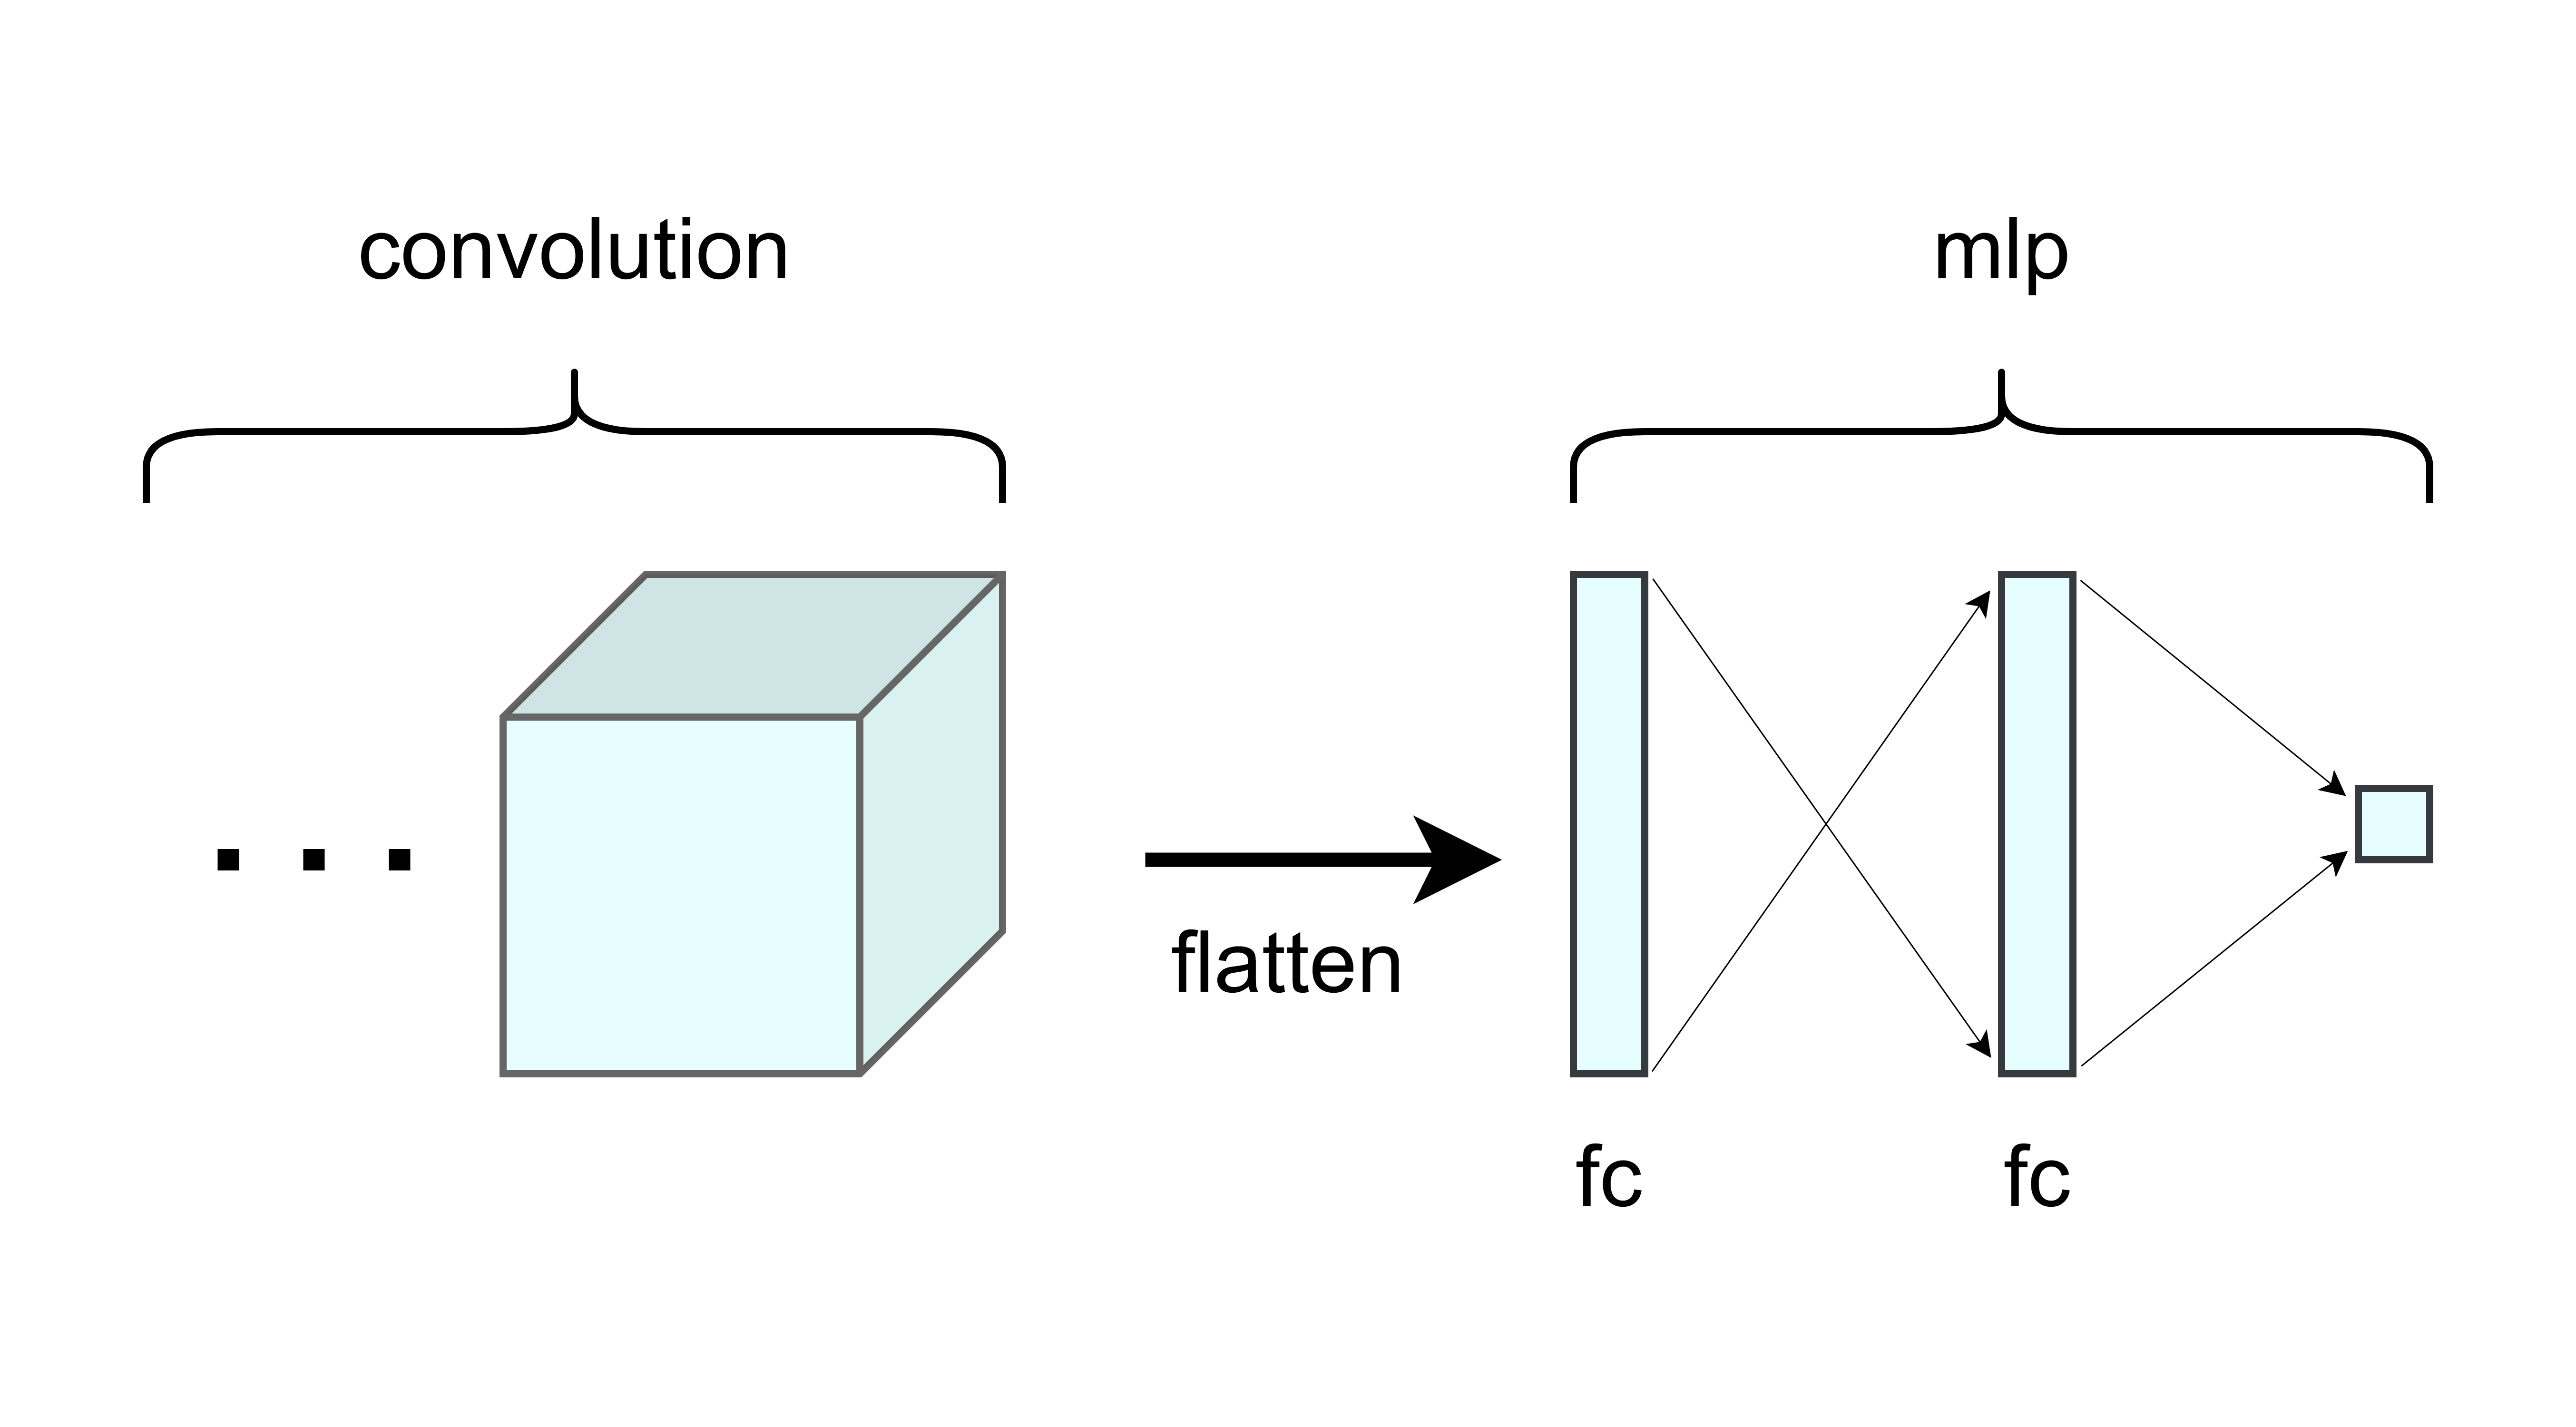
\includegraphics[scale=0.027]{fig1.png}
	\caption{A simple MLP after some convolution layers.}
	\label{fig:1}
\end{figure}
\subsubsection{Tensor contraction layer}
\label{subsubsec:tcl}
\textit{Tensor Contraction Layer} (TCL) \cite{r1} is a form of feature extraction and can also be used for embedding. The primary idea behind TCL is Tucker decomposition; by multiplying matrices to each mode of the input tensor, we can obtain a denser tensor. Figure \ref{fig:2-3} demonstrates the TCL process on a third-order tensor.


Given an input tensor $\mathcal{X} \in \mathbb{R}^{S_0\times I_1\times\dots\times I_N}$, a rank $(R_1,\dots,R_N)$ TCL on $\mathcal{X}$  is defined as :
\begin{align}
	\label{eq:tcl}
	&\hat{\mathcal{X}} = \left(V^{(1)},\dots,V^{(N)}\right)_{1:N} \mathcal{X}
	\nonumber\\
	&\hat{\mathcal{X}}_{[0]} = \mathcal{X}_{[0]} (V^{(1)}\otimes\dots\otimes V^{(N)})^T
\end{align}
where $S_0$ is the batch index and $V^{(i)} \in \mathbb{R}^{R_i\times I_i}$ is the TCL factor; The number of required parameters is calculated as :
\begin{align}
	\label{eq:tcl-parmeter}
	\sum_{i=1}^{N}R_i\times I_i
\end{align}
And the resulting tensor is of size $(S_0,R_1,\dots,R_N)$.
Compared to the FC version where the simple regression between these two tensors would require at least $\prod_{i=1}^{N}I_i\times R_i$ parameters.
%Considering an input tensor $\mathcal{T}$ of size 
%$(S_0,I_1,\dots,I_N)$ and a size  
%$(R_1,\dots,R_N)$ TCL, where $S_0$ is the size of the batch and $(I_i,R_i)$ is the shape of the matrix applied to mode $i$ of the tensor; The number of required parameters is calculated as :
%$\sum_{i=1}^{N}I_i\times R_i$; And the resulting tensor is of size 
%$(S_0,R_1,\dots,R_N)$. Compared to the FC version where the simple regression between these two tensors would require $\prod_{i=1}^{N}I_i\times R_i$ parameters.
\subsubsection{Tensor regression layer}
\label{subsubsec:trl}
\textit{Tensor Regression Layers} (TRL) \cite{r1} are a replacement for the FC regression layers. A simple regression that is the foundation of an MLP is a generalized inner product of $\mathcal{W}$ (Weight Tensor) with $\mathcal{X}$ (Input tensor). The idea behind TRL is to reconstruct $\mathcal{W}$ from a low-rank approximation of itself via Tucker decomposition. In Figure \ref{fig:2-3}, a TRL application in an MLP is provided. For the sake of simplicity, we considered a binary classification problem where the output of the inner product is a scalar. Similarly, if the desired output is a vector or even a tensor, $\mathcal{W}$ will be a higher-dimensional tensor to generate each mode of the output.


Given an input tensor $\mathcal{X} \in \mathbb{R}^{S_0\times I_1\times\dots\times I_N}$, output tensor $\mathcal{Y} \in \mathbb{R}^{S_0\times O}$, a rank $(R_1,\dots,R_N, R_{N+1})$ TRL on $\mathcal{X}$  is defined as:
\begin{align}
	\label{eq:trl}
	\mathcal{W} &= \left(U^{(1)},\dots,U^{(N)}, U^{(N+1)}\right)_{0:N+1} \mathcal{G}
	\nonumber\\
	\mathcal{Y} &=  \left\langle \mathcal{X}, \mathcal{W}\right\rangle_N
\end{align}
where $S_0$ is the batch index, $\forall i \hspace{1mm}U^{(i)} \in \mathbb{R}^{R_i\times I_i}$,
$U^{(N+1)} \in \mathbb{R}^{R_{N+1}\times O}$,
and $\mathcal{G} \in \mathbb{R}^{R_1\times\dots\times R_N\times O}$; The number of required parameters can be calculated as :
\begin{align}
	\label{eq:trl-parmeter}
	\prod_{i=1}^{N+1}R_i + \left(\sum_{i=1}^{N} R_i\times I_i + R_{N+1}\times O \right)
\end{align}
Compared to the FC version where the number of parameters is $O\times\prod_{i=1}^{N}I_i$.
\begin{figure}
	\centering
	\includegraphics[scale=0.023]{fig2-3.png}
	\caption{Tensor regression networks, replacement for FC layers. In $(a)$, A simple TCL is applied; Each mode $i$ of tensor $\mathcal{T}$ is multiplied by factor $\mathbf{A}^{(i)}$.
	In $(b)$, A TRL is applied; Generalized inner product of input tensor $\mathcal{T}$ and weight tensor $\mathcal{W}$ is calculated as the output tensor while considering a low rank approximation of weight tensor $\mathcal{W}$ in a tucker decomposed form. 
	}
	\label{fig:2-3}
\end{figure}
\section{Splitting approach}
\label{sec:splitting-approach}

Impressed by the Vision Transformer's patching and down-sampling methods, we can transform our input tensor into a thinner and higher-dimensional tensor that not only reduces the number of parameters for a TRL or TCL layer but also maintains accuracy. However, not every reshaping scheme to arbitrary higher orders and dimensions guarantees that the multi-linear structure is preserved and the accuracy is maintained. With a proper splitting scheme, the newly made tensor has a better physical interpretation than the flattened data. We introduced two splitting schemes, both of which are useful and could be used differently according to the network architecture. Figure \ref{fig:4} demonstrates the general splitting outline. Given a third-order tensor, if we split across each mode, the output is a sixth-order tensor where the first three modes correspond to the split index, and the next three modes are the split data.
\begin{figure}
	\centering
	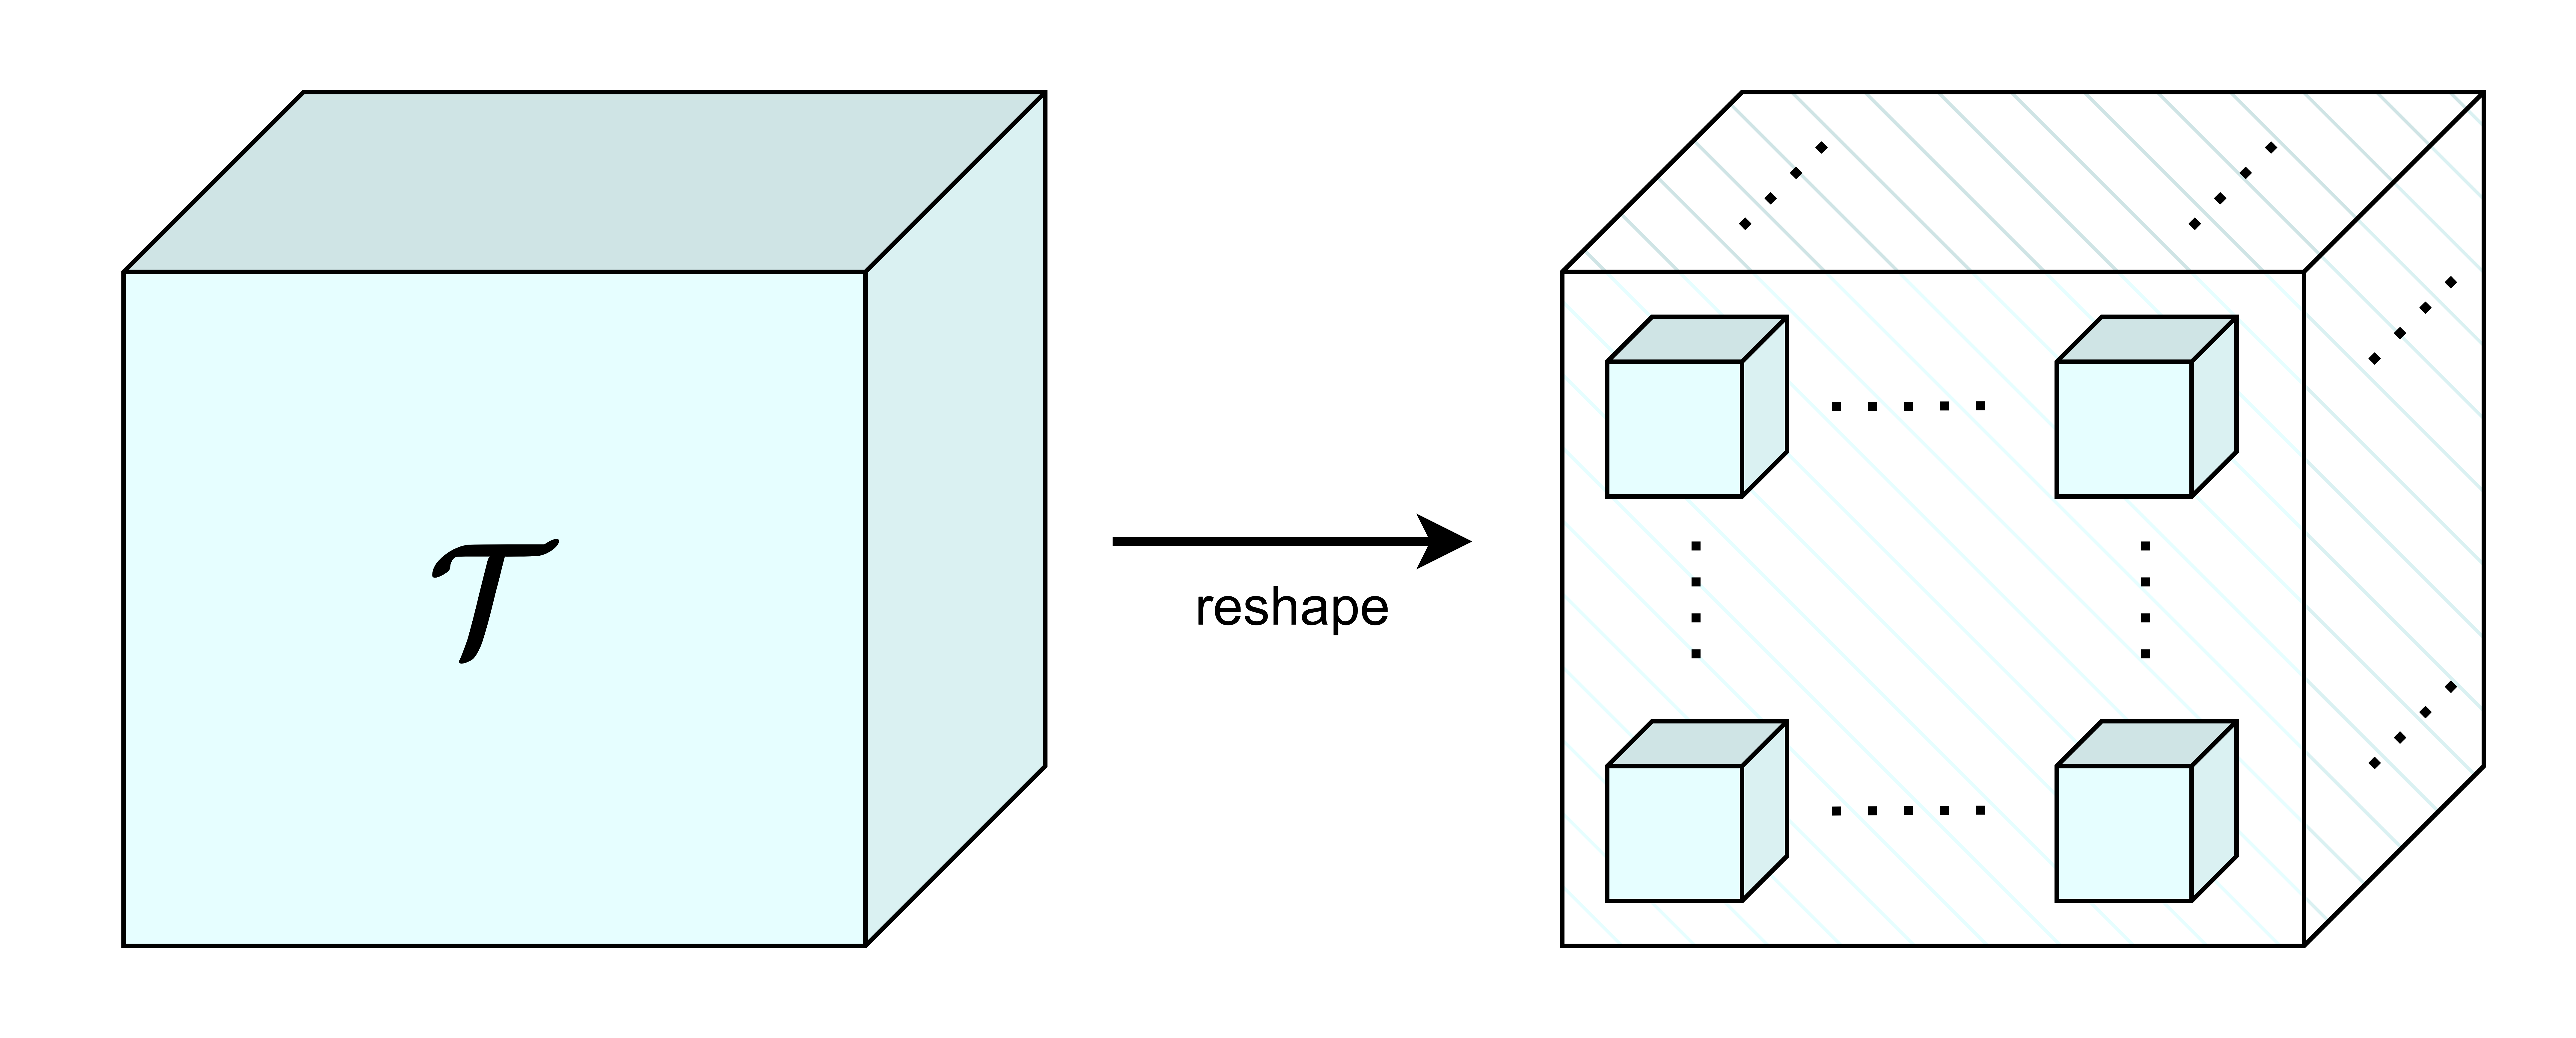
\includegraphics[scale=0.013]{fig4.png}
	\caption{
		An outline of reshaping to higher orders tensor.
	}
	\label{fig:4}
\end{figure}
\subsection{Attached splitting}
\label{subsec:attached-approach}

In attached splitting, every split is continues; That is if mode  $I_i$ of the input tensor $\mathcal{X}$ with length $n$ is to be split into two parts, then the split indices are $(0,\frac{n}{2})$ and $(\frac{n}{2}, n)$.
Figure 
\ref{fig:5} 
demonstrate the splitting process on a matrix. 

Given a tensor $\mathcal{T} \in \mathbb{R}^{I_1\times\dots\times I_N}$ and split sizes 
$\left(L_1,\dots,L_N\right)$, attached mapping of elements is done via:
\begin{align}
	\label{eq:map1}
	\mathcal{T}\left[i_1,\dots,i_N\right] \longrightarrow
	\mathcal{T}_a\left[
	\lfloor\frac{L_1\times i_1}{I_1}\rfloor,
	\dots,
	\lfloor\frac{L_N\times i_N}{I_N}\rfloor,
	i_1 \bmod{\frac{I_1}{L_1}},
	\dots,
	i_N \bmod{\frac{I_N}{L_N}},
	\right]
\end{align}
where $\mathcal{T}_a \in \mathbb{R}^{L_1\times\dots\times L_N\times \frac{I_1}{L_1}\times\dots\times \frac{I_N}{L_N}}$.
\subsection{Compressed splitting}
\label{subsec:copressed-splitting}

In compressed splitting, we incorporate the idea behind down sampling. If mode $I_i$ of input tensor $\mathcal{X}$ with length $n$ is to be split into $2$ part , different to the attached splitting, the indices are even-odd combinations; That is $\left\{
t | t \in (0,n) \land 
\left(t\bmod{2} = 0\right)
\right\}$
and 
$\left\{
t | t \in (0,n) \land 
\left(t\bmod{2} = 1\right)
\right\}$.

Given a tensor $\mathcal{T} \in \mathbb{R}^{I_1\times\dots\times I_N}$ and split sizes 
$\left(L_1,\dots,L_N\right)$, compressed mapping of elements is done via:
\begin{align}
	\label{eq:map2}
	\mathcal{T}\left[i_1,\dots,i_N\right] \longrightarrow
	\mathcal{T}_c\left[
	i_1 \bmod{L_1},
	\dots,
	i_N \bmod{L_N},
	\lfloor\frac{i_1}{L_1}\rfloor,
	\dots,
	\lfloor\frac{i_N}{L_N}\rfloor,
	\right]
\end{align}
where $\mathcal{T}_c \in \mathbb{R}^{L_1\times\dots\times L_N\times \frac{I_1}{L_1}\times\dots\times \frac{I_N}{L_N}}$.
\subsection{Method analysis}
\label{subsec:method-analysis}
Considering an input tensor $\mathcal{X}$ of size
$(S_0,I_1,\dots,I_N)$
, either reshaping would result in the tensor $\hat{\mathcal{X}}$ of size
$(S_0,L_1,\dots,L_N,\frac{I_1}{L_1}, \dots, \frac{I_N}{L_N})$. An example of each reshaping approach is shown in Figure \ref{fig:6-7-8} on a sample image.

In case of a $(r_1\dots,r_N, R_i,\dots,R_N)$ TCL, Since $L_i$s are usually small, the number of parameters required for them $\sum_{i=0}^{N}L_i\times r_i$ is also small; Similarly, $\frac{I_i}{L_i}$ is smaller than $I_i$ so the new desired $R_i$s is smaller than the previous $R_i$s and the total number of parameters can be calculated as:
\begin{align}
	\label{eq:reshape-parameter-tcl}
	\sum_{i=1}^{N}L_i\times r_i + \sum_{i=1}^{N} R_i \times \frac{I_i}{L_i}
\end{align}
which is ideally less than equation \ref{eq:tcl-parmeter} (Appendix \ref{proof-1} and \ref{subspace-tcl}).

In case of 
$(r_1,\dots,r_N, R_1,\dots,R_N,R_{N+1})$
TRL, the same logic as TCL \ref{eq:reshape-parameter-tcl}could also be applied. The total number of parameters in a new TRL is calculated as:
\begin{align}
	\label{eq:reshape-parameter-trl}
	\left(\prod_{i=1}^{N}r_i \prod_{i=1}^{N+1}R_i\right) + \left(\sum_{i=1}^{N}L_i\times r_i + \sum_{i=1}^{N} R_i \times \frac{I_i}{L_i} + R_{N+1}\times O\right)
\end{align} 
which is ideally less than equation \ref{eq:trl-parmeter} (Appendix \ref{proof-2} and \ref{subspace-trl}).
\begin{figure}
	\centering
	\includegraphics[scale=0.024]{fig5.png}
	\caption{
		$(a)$ attached splitting of a second-order tensor. $(b)$ compressed splitting of a second-order tensor. $(c)$ demonstration of stacking split chunks of a second-order tensor into a 4-order tensor.
	}
	\label{fig:5}
\end{figure}
\begin{figure}
	\centering
	\includegraphics[scale=0.03]{678.png}
	\caption{
		$(a)$ original sample image. $(b)$ reshaped sample image using attached approach. $(c)$ reshaped sample image using compressed approach. Input Image $\mathcal{T}\in \mathbb{R}^{C,H,W}$, only $H$ and $W$ indices have been split. 
	}
	\label{fig:6-7-8}
\end{figure}
\section{Experiments}
\label{sec:experiments}

	We conducted a series of experiments to assess the performance of our proposed framework. Our experiments were performed on a 
	GeForce RTX 4090, 13th Gen Intel(R) Core(TM) i9-13900K, 24 core, 24564MiB
	. Datasets \ref{table:datasets} MNIST, CIFAR10, and Tiny ImageNet-200 applied to ResNet50, ResNet101, VGG-19, and a classic CNN demonstrate that our methods can significantly reduce the number of parameters while maintaining or even improving classification accuracy. In Tables \ref{table:resnet_mnist_cifar10}, \ref{table:vgg_tiny}, and \ref{table:cnn_mnist}, parameters include only the classifier parameters. For a better representation of our methods, we ignored adaptive average pooling layers in all models. $^A$ and $^C$ are splitting approaches. Code of this project will be made publicly available at our github. 
	
		\begin{table}
		\centering
		\caption{
			Datasets information
		}
		\label{table:datasets}
		\begin{tabular}{c c c c}
			\toprule
			\textbf{Dataset} & \textbf{\# classes} & \textbf{\# training samples} & \textbf{\# testing samples} 
			\\
			\midrule
			 MNIST	& 10    &  60,000   &  10,000  \\
			\midrule
			CIFAR10	& 10  & 50,000   & 10,000   \\
			\midrule
			Tiny ImageNet	& 200  & 100,000  &  10,000 \\
			\bottomrule
		\end{tabular}
	\end{table}
	\begin{table}
		\centering
		\caption{
		\textbf{Performance evaluation of ResNet50 and ResNet101}, Our methods reduce the number of parameters by more than 90 \% while achieving near similar accuracy. More detailed Table(s) at (Appendix \ref{additional-tables}).
			}
		\label{table:resnet_mnist_cifar10}
		\begin{tabular}{c c c c c c}
			\toprule
			\textbf{Dataset} & \textbf{Model} & \textbf{TRL} & \textbf{Split} & \textbf{Parameters} & \textbf{Top-1 (\%)} \\
			\midrule
			\multirow{8}{*}{MNIST} & \multirow{4}{*}{Resnet50} &  Baseline &   & 737,290 & 97.25 \\ 
			& & (50,3,3,3) &   & 103,816 & 96.49 \\ 
			& & (1,1,1,20,1,1,4) & (2,2,2)\(^A\) & 20,612 & 98.56 \\ 
			& & (4,1,1,20,1,1,10) & (16,2,2)\(^C\) & 3,534 & 98.12 \\ 
			\cmidrule(lr){2-6}
			& \multirow{4}{*}{Resnet101} &  Baseline &   & 737,290 & 98.58 \\ 
			& & (50,3,3,3) &   & 103,816 & 97.42 \\ 
			& & (1,1,1,20,1,1,4) & (2,2,2)\(^C\) & 20,612 & 98.24 \\ 
			& & (4,1,1,20,1,1,10) & (16,2,2)\(^A\) & 3,534 & 98.40 \\ 
			\midrule
			\multirow{8}{*}{CIFAR10} & \multirow{4}{*}{Resnet50} &  Baseline &   & 737,290 & 90.71 \\ 
			& & (50,3,3,3) &   & 103,816 & 90.41 \\ 
			& & (1,1,1,100,1,1,10) & (2,2,2)\(^C\) & 103,512 & 92.58 \\ 
			& & (4,1,1,10,1,1,4) & (16,2,2)\(^A\) & 1,386 & 90.44 \\ 
			\cmidrule(lr){2-6}
			& \multirow{4}{*}{Resnet101} &  Baseline &   & 737,290 & 92.67 \\ 
			& & (50,3,3,3) &   & 103,816 & 90.30 \\ 
			& & (1,1,1,100,1,1,10) & (2,2,2)\(^C\) & 103,512 & 91.85 \\ 
			& & (4,1,1,10,1,1,4) & (16,2,2)\(^A\) & 1,386 & 92.43 \\ 
			\bottomrule
		\end{tabular}
	\end{table}
	\begin{table}
		\centering
		\caption{
			\textbf{Tiny ImageNet-200 performance on VGG-19},
			 Given extreme number of classifier parameters for a VGG-19 model, we applied TCL layers before TRL layers. More detailed Table(s) at (Appendix \ref{additional-tables}). 
			}
		\label{table:vgg_tiny}
		\begin{tabular}{c c c c c c}
			\toprule
			\textbf{TCL} & \textbf{TRL} & \textbf{Split} & \textbf{Parameters} & \textbf{Top-1(\%)} & \textbf{Top-5(\%)} \\
			\midrule
			 Baseline &   &   & 93,102,280 & 63.66 & 84.16 \\ 
			(512,6,6) & (512,6,6,200) &   & 4,250,832 & 67.32 & 87.87 \\ 
			(2,2,2,256,1,1) & (1,1,1,256,1,1,200) & (2,2,2)\(^A\) & 666,714 & 68.91 & 88.16 \\ 
			(6,2,2,64,3,3) & (4,2,2,64,1,1,200) & (8,2,2)\(^C\) & 253,104 & 68.29 & 88.34 \\ 
			\bottomrule
		\end{tabular}
	\end{table}
	\begin{table}
		\centering
		\caption{
			\textbf{Classic CNN on MNIST},  Our methods are dependent on a good convolutional foundation. More detailed Table(s) at (Appendix \ref{additional-tables}). 
			}
		\label{table:cnn_mnist}
		\begin{tabular}{c c c c c}
			\toprule
			\textbf{TCL} & \textbf{TRL} & \textbf{Split} & \textbf{Parameters} & \textbf{Top-1(\%)} \\
			\midrule
			Baseline &   &   & 4,729,866 & 98.14 \\ 
			(128,6,6) & (128,6,6,10) &   & 79,092 & 95.62 \\ 
			(2,1,1,64,6,6) & (2,1,1,64,6,6,10) & (2,1,1)\(^A\) & 54,528 & 97.11 \\ 
			(2,1,1,64,6,6) & (2,1,1,64,6,6,10) & (2,1,1)\(^C\) & 54,528 & 97.12 \\ 
			\bottomrule
		\end{tabular}
	\end{table}
%	\subsection{Analysis}
%	
	Our framework performs exceptionally well compared to traditional TCL TRL and baseline models across various datasets and architectures. Notably, our approach significantly reduces the number of parameters without acutely compromising accuracy. 
	In Figure \ref{fig:9}, loss and accuracy of selected models and datasets are plotted. 
	The \textbf{ablation study} is carried out in the Appendix \ref{ablation-study}.
%	
	\begin{figure}[h!]
		\centering
		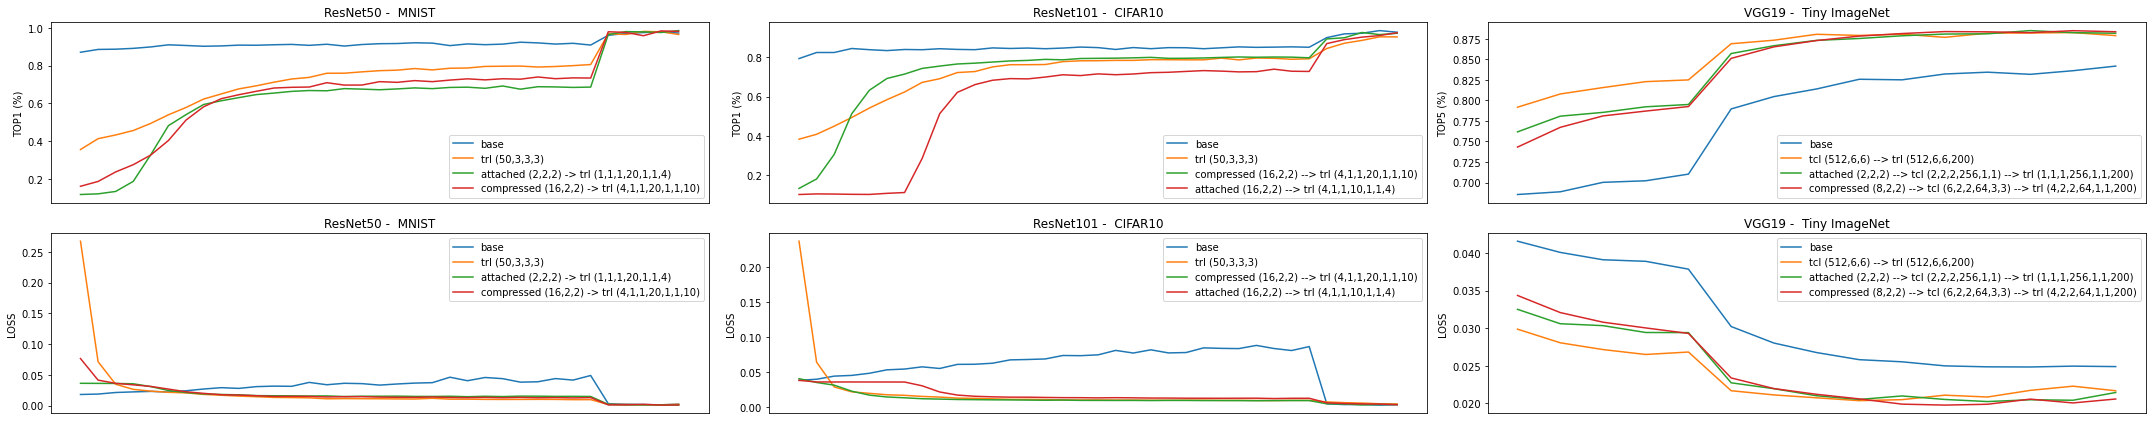
\includegraphics[width=0.85\textwidth, height=0.3\textheight]{plot.png}
		\caption{Accuracy and loss plots (Baseline, TCL TRL, Our Method)
		}
		\label{fig:9}
	\end{figure}

	
\section{Conclusion}
\label{sec:conclusion}
Although methods like TRL and TCL can achieve nearly similar accuracy while preserving the multi-modal structure of the data and reducing the number of classifier parameters, these methods perform poorly when the approximated rank is too low. We introduced SATURN, a framework that maintains the quality of the network and reduces the number of classifier parameters by more than 95\%. Our experiment, evaluated on CIFAR10, MNIST, and Tiny ImageNet-200 and applied to ResNet50, ResNet101, VGG19, and classic CNNs, demonstrates that by splitting the input tensor via an approach that does not disturb the multi-linear structure of the data, a TCL or TRL with fewer parameters can be performed while maintaining accuracy. While our framework and similar approaches offer theoretical advantages, they currently do not exhibit the expected speed. This limitation underscores the primary challenge in applying tensor methods to models, as the development of optimal implementations remains a pending task.


%\section{General formatting instructions}
%\label{gen_inst}
%
%
%
%The text must be confined within a rectangle 5.5~inches (33~picas) wide and
%9~inches (54~picas) long. The left margin is 1.5~inch (9~picas).  Use 10~point
%type with a vertical spacing (leading) of 11~points.  Times New Roman is the
%preferred typeface throughout, and will be selected for you by default.
%Paragraphs are separated by \nicefrac{1}{2}~line space (5.5 points), with no
%indentation.
%
%
%The paper title should be 17~point, initial caps/lower case, bold, centered
%between two horizontal rules. The top rule should be 4~points thick and the
%bottom rule should be 1~point thick. Allow \nicefrac{1}{4}~inch space above and
%below the title to rules. All pages should start at 1~inch (6~picas) from the
%top of the page.
%
%
%For the final version, authors' names are set in boldface, and each name is
%centered above the corresponding address. The lead author's name is to be listed
%first (left-most), and the co-authors' names (if different address) are set to
%follow. If there is only one co-author, list both author and co-author side by
%side.
%
%
%Please pay special attention to the instructions in Section \ref{others}
%regarding figures, tables, acknowledgments, and references.
%
%
%\section{Headings: first level}
%\label{headings}
%
%
%All headings should be lower case (except for first word and proper nouns),
%flush left, and bold.
%
%
%First-level headings should be in 12-point type.
%
%
%\subsection{Headings: second level}
%
%
%Second-level headings should be in 10-point type.
%
%
%\subsubsection{Headings: third level}
%
%
%Third-level headings should be in 10-point type.
%
%
%\paragraph{Paragraphs}
%
%
%There is also a \verb+\paragraph+ command available, which sets the heading in
%bold, flush left, and inline with the text, with the heading followed by 1\,em
%of space.
%
%
%\section{Citations, figures, tables, references}
%\label{others}
%
%
%These instructions apply to everyone.
%
%
%\subsection{Citations within the text}
%
%
%The \verb+natbib+ package will be loaded for you by default.  Citations may be
%author/year or numeric, as long as you maintain internal consistency.  As to the
%format of the references themselves, any style is acceptable as long as it is
%used consistently.
%
%
%The documentation for \verb+natbib+ may be found at
%\begin{center}
%  \url{http://mirrors.ctan.org/macros/latex/contrib/natbib/natnotes.pdf}
%\end{center}
%Of note is the command \verb+\citet+, which produces citations appropriate for
%use in inline text.  For example,
%\begin{verbatim}
%   \citet{hasselmo} investigated\dots
%\end{verbatim}
%produces
%\begin{quote}
%  Hasselmo, et al.\ (1995) investigated\dots
%\end{quote}
%
%
%If you wish to load the \verb+natbib+ package with options, you may add the
%following before loading the \verb+neurips_2024+ package:
%\begin{verbatim}
%   \PassOptionsToPackage{options}{natbib}
%\end{verbatim}
%
%
%If \verb+natbib+ clashes with another package you load, you can add the optional
%argument \verb+nonatbib+ when loading the style file:
%\begin{verbatim}
%   \usepackage[nonatbib]{neurips_2024}
%\end{verbatim}
%
%
%As submission is double blind, refer to your own published work in the third
%person. That is, use ``In the previous work of Jones et al.\ [4],'' not ``In our
%previous work [4].'' If you cite your other papers that are not widely available
%(e.g., a journal paper under review), use anonymous author names in the
%citation, e.g., an author of the form ``A.\ Anonymous'' and include a copy of the anonymized paper in the supplementary material.
%
%
%\subsection{Footnotes}
%
%
%Footnotes should be used sparingly.  If you do require a footnote, indicate
%footnotes with a number\footnote{Sample of the first footnote.} in the
%text. Place the footnotes at the bottom of the page on which they appear.
%Precede the footnote with a horizontal rule of 2~inches (12~picas).
%
%
%Note that footnotes are properly typeset \emph{after} punctuation
%marks.\footnote{As in this example.}
%
%
%\subsection{Figures}
%
%
%\begin{figure}
%  \centering
%  \fbox{\rule[-.5cm]{0cm}{4cm} \rule[-.5cm]{4cm}{0cm}}
%  \caption{Sample figure caption.}
%\end{figure}
%
%
%All artwork must be neat, clean, and legible. Lines should be dark enough for
%purposes of reproduction. The figure number and caption always appear after the
%figure. Place one line space before the figure caption and one line space after
%the figure. The figure caption should be lower case (except for first word and
%proper nouns); figures are numbered consecutively.
%
%
%You may use color figures.  However, it is best for the figure captions and the
%paper body to be legible if the paper is printed in either black/white or in
%color.
%
%
%\subsection{Tables}
%
%
%All tables must be centered, neat, clean and legible.  The table number and
%title always appear before the table.  See Table~\ref{sample-table}.
%
%
%Place one line space before the table title, one line space after the
%table title, and one line space after the table. The table title must
%be lower case (except for first word and proper nouns); tables are
%numbered consecutively.
%
%
%Note that publication-quality tables \emph{do not contain vertical rules.} We
%strongly suggest the use of the \verb+booktabs+ package, which allows for
%typesetting high-quality, professional tables:
%\begin{center}
%  \url{https://www.ctan.org/pkg/booktabs}
%\end{center}
%This package was used to typeset Table~\ref{sample-table}.
%
%
%\begin{table}
%  \caption{Sample table title}
%  \label{sample-table}
%  \centering
%  \begin{tabular}{lll}
%    \toprule
%    \multicolumn{2}{c}{Part}                   \\
%    \cmidrule(r){1-2}
%    Name     & Description     & Size ($\mu$m) \\
%    \midrule
%    Dendrite & Input terminal  & $\sim$100     \\
%    Axon     & Output terminal & $\sim$10      \\
%    Soma     & Cell body       & up to $10^6$  \\
%    \bottomrule
%  \end{tabular}
%\end{table}
%
%\subsection{Math}
%Note that display math in bare TeX commands will not create correct line numbers for submission. Please use LaTeX (or AMSTeX) commands for unnumbered display math. (You really shouldn't be using \$\$ anyway; see \url{https://tex.stackexchange.com/questions/503/why-is-preferable-to} and \url{https://tex.stackexchange.com/questions/40492/what-are-the-differences-between-align-equation-and-displaymath} for more information.)
%
%\subsection{Final instructions}
%
%Do not change any aspects of the formatting parameters in the style files.  In
%particular, do not modify the width or length of the rectangle the text should
%fit into, and do not change font sizes (except perhaps in the
%\textbf{References} section; see below). Please note that pages should be
%numbered.
%
%
%\section{Preparing PDF files}
%
%
%Please prepare submission files with paper size ``US Letter,'' and not, for
%example, ``A4.''
%
%
%Fonts were the main cause of problems in the past years. Your PDF file must only
%contain Type 1 or Embedded TrueType fonts. Here are a few instructions to
%achieve this.
%
%
%\begin{itemize}
%
%
%\item You should directly generate PDF files using \verb+pdflatex+.
%
%
%\item You can check which fonts a PDF files uses.  In Acrobat Reader, select the
%  menu Files$>$Document Properties$>$Fonts and select Show All Fonts. You can
%  also use the program \verb+pdffonts+ which comes with \verb+xpdf+ and is
%  available out-of-the-box on most Linux machines.
%
%
%\item \verb+xfig+ "patterned" shapes are implemented with bitmap fonts.  Use
%  "solid" shapes instead.
%
%
%\item The \verb+\bbold+ package almost always uses bitmap fonts.  You should use
%  the equivalent AMS Fonts:
%\begin{verbatim}
%   \usepackage{amsfonts}
%\end{verbatim}
%followed by, e.g., \verb+\mathbb{R}+, \verb+\mathbb{N}+, or \verb+\mathbb{C}+
%for $\mathbb{R}$, $\mathbb{N}$ or $\mathbb{C}$.  You can also use the following
%workaround for reals, natural and complex:
%\begin{verbatim}
%   \newcommand{\RR}{I\!\!R} %real numbers
%   \newcommand{\Nat}{I\!\!N} %natural numbers
%   \newcommand{\CC}{I\!\!\!\!C} %complex numbers
%\end{verbatim}
%Note that \verb+amsfonts+ is automatically loaded by the \verb+amssymb+ package.
%
%
%\end{itemize}
%
%
%If your file contains type 3 fonts or non embedded TrueType fonts, we will ask
%you to fix it.
%
%
%\subsection{Margins in \LaTeX{}}
%
%
%Most of the margin problems come from figures positioned by hand using
%\verb+\special+ or other commands. We suggest using the command
%\verb+\includegraphics+ from the \verb+graphicx+ package. Always specify the
%figure width as a multiple of the line width as in the example below:
%\begin{verbatim}
%   \usepackage[pdftex]{graphicx} ...
%   \includegraphics[width=0.8\linewidth]{myfile.pdf}
%\end{verbatim}
%See Section 4.4 in the graphics bundle documentation
%(\url{http://mirrors.ctan.org/macros/latex/required/graphics/grfguide.pdf})
%
%
%A number of width problems arise when \LaTeX{} cannot properly hyphenate a
%line. Please give LaTeX hyphenation hints using the \verb+\-+ command when
%necessary.

%\begin{ack}
%	TODO
%%Use unnumbered first level headings for the acknowledgments. All acknowledgments
%%go at the end of the paper before the list of references. Moreover, you are required to declare
%%funding (financial activities supporting the submitted work) and competing interests (related financial activities outside the submitted work).
%%More information about this disclosure can be found at: \url{https://neurips.cc/Conferences/2024/PaperInformation/FundingDisclosure}.
%%
%%
%%Do {\bf not} include this section in the anonymized submission, only in the final paper. You can use the \texttt{ack} environment provided in the style file to automatically hide this section in the anonymized submission.
%\end{ack}

%\section*{References}

\bibliographystyle{unsrt}
\bibliography{ref}

%References follow the acknowledgments in the camera-ready paper. Use unnumbered first-level heading for
%the references. Any choice of citation style is acceptable as long as you are
%consistent. It is permissible to reduce the font size to \verb+small+ (9 point)
%when listing the references.
%Note that the Reference section does not count towards the page limit.
%\medskip
%
%
%{
%\small
%
%
%[1] Alexander, J.A.\ \& Mozer, M.C.\ (1995) Template-based algorithms for
%connectionist rule extraction. In G.\ Tesauro, D.S.\ Touretzky and T.K.\ Leen
%(eds.), {\it Advances in Neural Information Processing Systems 7},
%pp.\ 609--616. Cambridge, MA: MIT Press.
%
%
%[2] Bower, J.M.\ \& Beeman, D.\ (1995) {\it The Book of GENESIS: Exploring
%  Realistic Neural Models with the GEneral NEural SImulation System.}  New York:
%TELOS/Springer--Verlag.
%
%
%[3] Hasselmo, M.E., Schnell, E.\ \& Barkai, E.\ (1995) Dynamics of learning and
%recall at excitatory recurrent synapses and cholinergic modulation in rat
%hippocampal region CA3. {\it Journal of Neuroscience} {\bf 15}(7):5249-5262.
%}


%%%%%%%%%%%%%%%%%%%%%%%%%%%%%%%%%%%%%%%%%%%%%%%%%%%%%%%%%%%%

\appendix

%\section{Appendix / supplemental material}
%Optionally include supplemental material (complete proofs, additional experiments and plots) in appendix.
%All such materials \textbf{SHOULD be included in the main submission.}

%\section{TCL}
%\label{A-tcl}
%Given an input tensor $\mathcal{X} \in \mathbb{R}^{S_0\times I_1\times\dots\times I_N}$, a rank $(R_1,\dots,R_N)$ TCL on $\mathcal{X}$  is defined as :
%
%\begin{align}
%	\label{eq:tcl2}
%	&\hat{\mathcal{X}} = \left(V^{(1)},\dots,V^{(N)}\right)_{1:N} \mathcal{X}
%	\nonumber\\
%	&\hat{\mathcal{X}}_{[0]} = \mathcal{X}_{[0]} (V^{(1)}\otimes\dots\otimes V^{(N)})^T
%\end{align}
%
%
%where $S_0$ is the batch index and $V^{(i)} \in \mathbb{R}^{R_i\times I_i}$.
%
%\section{TRL}
%\label{A-trl}
%Given an input tensor $\mathcal{X} \in \mathbb{R}^{S_0\times I_1\times\dots\times I_N}$, output tensor $\mathcal{Y} \in \mathbb{R}^{S_0\times O}$, a rank $(R_1,\dots,R_N, R_{N+1})$ TRL on $\mathcal{X}$  is defined as:
%
%\begin{align}
%	\label{eq:trl2}
%	\mathcal{W} &= \left(U^{(1)},\dots,U^{(N)}, U^{(N+1)}\right)_{0:N+1} \mathcal{G}
%	\nonumber\\
%	\mathcal{Y} &=  \left\langle \mathcal{X}, \mathcal{W}\right\rangle_N
%\end{align}
%
%where $S_0$ is the batch index, $\forall i \hspace{1mm}U^{(i)} \in \mathbb{R}^{R_i\times I_i}$,
%$U^{(N+1)} \in \mathbb{R}^{R_{N+1}\times O}$,
%and $\mathcal{G} \in \mathbb{R}^{R_1\times\dots\times R_N\times O}$.

\section{Method analysis on TCL}
\label{proof-1}
As stated in subsection \ref{subsec:method-analysis}, 
equation \ref{eq:reshape-parameter-tcl}, the number of required parameters for a TCL on our framework is ideally less than equation \ref{eq:tcl-parmeter}. Given $\mathcal{T} \in \mathbb{R}^{I_1\times\dots\times I_N}$ and $\hat{\mathcal{T}} \in \mathbb{R}^{L_1\times\dots\times L_N\times \frac{I_1}{L_1}\times\dots\times\frac{I_N}{L_N}}$, ideally a rank $(r_1,\dots,r_N, \hat{R}_1, \dots, \hat{R}_N)$ TCL on $\hat{\mathcal{T}}$ has less parameters than a rank $(R_1,\dots,R_N)$ TCL on $\mathcal{T}$. Since TCL ranks are arbitrary values, one can choose these ranks in a way that inequality \ref{eq:proof-1-14} does not hold.
\begin{align}
	\label{eq:proof-1-14}
	\sum_{i=1}^{N}L_i\times r_i + \sum_{i=1}^{N} \hat{R}_i \times \frac{I_i}{L_i} \leq
	\sum_{i=1}^{N}R_i\times I_i
\end{align}
%\begin{proof}[\textbf{ideal}]
\begin{proof}
	We prove that given ideal ranks, inequality \ref{eq:proof-1-14} holds. 
	
	Assume $\forall i \hspace{2mm}\hat{R}_i \leq R_i$, then:
	\begin{align}
		\label{eq:proof-1-15}
		\sum_{i=1}^{N} \hat{R}_i \times \frac{I_i}{L_i} \leq \sum_{i=1}^{N}R_i\times I_i \hspace{10mm}&  \forall i \hspace{2mm} L_i \geq 1
	\end{align}
	Consider $\alpha$ as:
	\begin{align}
		\label{eq:proof-1-16}
		\nonumber
		\alpha &= \sum_{i=1}^{N}R_i\times I_i - \sum_{i=1}^{N} \hat{R}_i \times \frac{I_i}{L_i}
		\\
		&= \sum_{i=1}^{N} (R_i - \frac{\hat{R}_i}{L_i})I_i
	\end{align}
	Then as long as the first part of equation \ref{eq:reshape-parameter-tcl} is less than $\alpha$, the inequality \ref{eq:proof-1-14} holds.
	\begin{align}
		\label{eq:proof-1-17}
		\sum_{i=0}^{N} r_i\times L_i \leq \alpha
	\end{align}
	Given the assumption and the inequality \ref{eq:proof-1-17}:
	\begin{align}
		\label{eq:proof-1-18}
		\sum_{i=1}^{N}L_i\times r_i + \sum_{i=1}^{N} \hat{R}_i \times \frac{I_i}{L_i} &\leq
		\alpha + \sum_{i=1}^{N} \hat{R}_i \times \frac{I_i}{L_i}
		\nonumber\\
		&\leq \sum_{i=1}^{N}R_i\times I_i - \sum_{i=1}^{N} \hat{R}_i \times \frac{I_i}{L_i} + \sum_{i=1}^{N} \hat{R}_i \times \frac{I_i}{L_i}
		\nonumber\\
		&\leq \sum_{i=1}^{N}R_i\times I_i
	\end{align}
Therefore, with ideal ranks, $\forall i \hspace{2mm}\hat{R}_i \leq R_i$ and $\sum_{i=0}^{N} r_i\times L_i \leq \alpha$, inequality \ref{eq:proof-1-14} holds. Given no ideal or some ideal ranks, there is no guarantee that inequality \ref{eq:proof-1-14} holds without further constraints. 
\end{proof}

%Given no ideal, or some ideal ranks, there is no guarantee that inequality \ref{eq:proof-1-14} holds without further constraints. We will briefly discuss some ideal settings for semi ideal ranks.  
%
%\begin{proof}[\textbf{semi ideal}] 
%	We prove that given semi ideal ranks, inequality \ref{eq:proof-1-14} holds. 
%	
%	Assume $\forall i \hspace{2mm}\hat{R}_i > R_i$, then:
%	\begin{align}
%		\label{eq:proof-1-19}
%		k_i = \hat{R}_i - R_i \hspace{10mm}&  \forall i
%	\end{align}
%	We can consider:
%	\begin{align}
%		\label{eq:proof-1-20}
%		\sum_{i=1}^{N} \hat{R}_i \times \frac{I_i}{L_i} = \sum_{i=1}^{N} R_i \times \frac{I_i}{L_i} + \sum_{i=1}^{N} k_i \times \frac{I_i}{L_i}
%	\end{align}
%	Consider $\beta$ as:
%	\begin{align}
%		\label{eq:proof-1-21}
%		\beta &= \sum_{i=1}^{N} R_i \times I_i - \sum_{i=1}^{N} R_i \times \frac{I_i}{L_i}
%		\nonumber\\
%		&= \sum_{i=1}^{N} R_i \times I_i \times (1 - \frac{1}{L_i})
%	\end{align}
%	Then as long as the second part of equations \ref{eq:proof-1-20} is less than $\beta$, the inequality \ref{eq:proof-1-15} holds.
%	\begin{align}
%		\label{eq:proof-1-22}
%		\sum_{i=1}^{N} k_i \times \frac{I_i}{L_i} \leq \beta
%	\end{align}
%Given the assumption and the inequality \ref{eq:proof-1-22}:
%\begin{align}
%	\label{eq:proof-1-23}
%	\sum_{i=1}^{N} \hat{R}_i \times \frac{I_i}{L_i} &= \sum_{i=1}^{N} R_i \times \frac{I_i}{L_i} + \sum_{i=1}^{N} k_i \times \frac{I_i}{L_i}
%	\nonumber \\
%	&\leq \sum_{i=1}^{N} R_i \times \frac{I_i}{L_i} + \beta 
%	\nonumber\\
%	&\leq  \sum_{i=1}^{N} R_i \times \frac{I_i}{L_i} + \sum_{i=1}^{N} R_i \times I_i - \sum_{i=1}^{N} R_i \times \frac{I_i}{L_i}
%	\nonumber\\
%	&\leq  \sum_{i=1}^{N} R_i \times I_i
%\end{align}
%Therefore, with ideal splits and $\sum_{i=1}^{N} k_i \times \frac{I_i}{L_i} \leq \beta$ , inequality \ref{eq:proof-1-15} holds. The rest of the proof is similar to \textit{\textbf{ideal}} case.
%\end{proof} 
%
%We will now prove that as long as the only existed semi-ideal ranks, follow the rule above, inequality \ref{eq:proof-1-14} can hold.
% 
%\begin{proof}[\textbf{semi ideal}]
%	We prove that given just some ideal ranks, inequality \ref{eq:proof-1-14} holds.
%	
%	 Assume $\exists j \hspace{2mm}\hat{R}_j > R_j$, then:
%	 \begin{align}
%	 	\label{eq:proof-1-24}
%	 	k_j = \hat{R}_j - R_j \hspace{10mm}&  \forall j \hspace{2mm}s.t \hspace{2mm} \hat{R}_j > R_j
%	 \end{align}
% We can consider $N_1 = \left\{\forall i \hspace{1mm}|\hspace{1mm} \hat{R}_i \leq i\right\}$ and $N_2 = \left\{\forall j \hspace{1mm}|\hspace{1mm} \hat{R}_j > j\right\}$ : 
% \begin{align}
% 	\label{eq:proof-1-25}
% 	\sum_{i=1}^{N} \hat{R}_i \times \frac{I_i}{L_i} &= \sum_{i\in N_1} \hat{R}_i \times \frac{I_i}{L_i} +  \sum_{j\in N_2} \hat{R}_j \times \frac{I_j}{L_j}
% 	\nonumber\\
% 	&\leq 
% 	\sum_{i\in N_1} R_i \times I_i +  \sum_{j\in N_2} \hat{R}_j \times \frac{I_j}{L_j}
% 	\nonumber \\
% 	&\leq 
% 	\sum_{i\in N_1} R_i \times I_i +  \sum_{j\in N_2} R_j \times \frac{I_j}{L_j} + \sum_{j\in N_2} k_j \times \frac{I_j}{L_j}
% \end{align}
%Consider $\beta$ as:
%\begin{align}
%	\label{eq:proof-1-26}
%	\beta &= \sum_{i = 1}^{N} R_i \times I_i - \sum_{i\in N_1} R_i \times I_i +  \sum_{j\in N_2} R_j \times \frac{I_j}{L_j}
%	\nonumber\\
%	&= \sum_{i \in N_1} R_i \times I_i + \sum_{j \in N_2} R_j \times I_j - \sum_{i\in N_1} R_i \times I_i +  \sum_{j\in N_2} R_j \times \frac{I_i}{L_i}
%	\nonumber\\
%	&= \sum_{j \in N_2} R_j \times I_j -  \sum_{j\in N_2} R_j \times \frac{I_i}{L_i}
%	\nonumber\\
%	&= \sum_{j \in N_2} R_j \times I_j \times (1 - \frac{1}{L_j})
%\end{align}
%Then as long as the last part of inequality \ref{eq:proof-1-25} is less than $\beta$, the inequality \ref{eq:proof-1-15} holds.
%\begin{align}
%	\label{eq:proof-1-27}
%	 \sum_{j\in N_2} k_j \times \frac{I_j}{L_j} \leq \beta
%\end{align}
%Given the assumption and the inequality \ref{eq:proof-1-27}:
%\begin{align}
%	\label{eq:proof-1-28}
%	\sum_{i=1}^{N} \hat{R}_i \times \frac{I_i}{L_i} &\leq
%	\sum_{i\in N_1} R_i \times I_i +  \sum_{j\in N_2} R_j \times \frac{I_j}{L_j} + \sum_{j\in N_2} k_j \times \frac{I_j}{L_j} 
%	\nonumber\\
%	&\leq
%	\sum_{i\in N_1} R_i \times I_i +  \sum_{j\in N_2} R_j \times \frac{I_j}{L_j} + \beta
%	\nonumber\\
%	&\leq
%	\sum_{i\in N_1} R_i \times I_i +  \sum_{j\in N_2} R_j \times \frac{I_j}{L_j} + \sum_{j \in N_2} R_j \times I_j -  \sum_{j\in N_2} R_j \times \frac{I_i}{L_i}
%	\nonumber\\
%	&\leq
%	\sum_{i\in N_1} R_i \times I_i +  \sum_{j \in N_2} R_j \times I_j
%	\nonumber \\
%	&\leq 
%	\sum_{i = 1}^{N}R_i \times I_i
%\end{align}
%Therefore, with ideal splits as long as the existed semi ideal ranks follow inequality \ref{eq:proof-1-27}, inequality \ref{eq:proof-1-15} holds. The rest of the proof is similar to \textit{\textbf{ideal}} case.
%\end{proof}

\section{Method analysis on TRL}
\label{proof-2}
As stated in subsection \ref{subsec:method-analysis}, equation \ref{eq:reshape-parameter-trl}, the number of required parameters for a TRL on our framework is ideally less than equations \ref{eq:trl-parmeter}. Given $\mathcal{T} \in \mathbb{R}^{S_0, I_1\times\dots\times I_N}$ and $\hat{\mathcal{T}} \in \mathbb{R}^{S_0, L_1\times\dots\times L_N\times \frac{I_1}{L_1}\times\dots\times\frac{I_N}{L_N}}$, and output $\mathcal{Y} \in \mathbb{R}^{S_0\times O}$, ideally a rank $(r_1,\dots,r_N, \hat{R}_1, \dots, \hat{R}_N, \hat{R}_{N+1})$ TRL on $\hat{\mathcal{T}}$ has less parameters than a rank $(R_1,\dots,R_N, R_{N+1})$ TRL on $\mathcal{T}$. Since TRL ranks are arbitrary values, one can choose these ranks in a way that inequality \ref{eq:proof-2-29} does not hold.
\begin{align}
	\label{eq:proof-2-29}
	\prod_{i=1}^{N}r_i \prod_{i=1}^{N+1}\hat{R}_i + \sum_{i=1}^{N}L_i\times r_i + \sum_{i=1}^{N} \hat{R}_i \times \frac{I_i}{L_i} + \hat{R}_{N+1}\times O \leq
	\prod_{i=1}^{N+1}R_i + \sum_{i=1}^{N} R_i\times I_i + R_{N+1}\times O 
\end{align}
%\begin{proof}[\textbf{ideal}]
\begin{proof}
	We prove that given ideal ranks, inequality \ref{eq:proof-2-29} holds. 
	
	Assume $\forall i \hspace{2mm}\hat{R}_i \leq R_i$, then:
	\begin{align}
		\label{eq:proof-2-30}
		\sum_{i=1}^{N} \hat{R}_i \times \frac{I_i}{L_i}  + \hat{R}_{N+1}\times O\leq \sum_{i=1}^{N}R_i\times I_i + R_{N+1}\times O \hspace{10mm}&  \forall i \hspace{2mm} L_i \geq 1
	\end{align}
	Consider $\alpha_1$ as:
	\begin{align}
		\label{eq:proof-2-31}
		\alpha_1 &= \sum_{i=1}^{N}R_i\times I_i + R_{N+1}\times O - \sum_{i=1}^{N} \hat{R}_i \times \frac{I_i}{L_i}  + \hat{R}_{N+1}\times O
		\nonumber\\
		&= \sum_{i=1}^{N}(R_i - \frac{\hat{R}_i}{L_i})\times I_i + (R_{N+1} - \hat{R}_{N+1})\times O
	\end{align}
	Then as long as the second part of equation \ref{eq:reshape-parameter-trl} is less than $\alpha_1$,
	\begin{align}
		\label{eq:proof-2-32}
		\sum_{i=1}^{N}L_i\times r_i \leq \alpha_1
	\end{align}
It proves that :
	\begin{align}
		\label{eq:proof-2-33}
		&\sum_{i=1}^{N}L_i\times r_i + \sum_{i=1}^{N} \hat{R}_i \times \frac{I_i}{L_i} + \hat{R}_{N+1}\times O 
		\nonumber\\
		&\leq
		\alpha_1 + \sum_{i=1}^{N} \hat{R}_i \times \frac{I_i}{L_i} + \hat{R}_{N+1}\times O 
		\nonumber\\
		&\leq
		\sum_{i=1}^{N}R_i\times I_i + R_{N+1}\times O - \sum_{i=1}^{N} \hat{R}_i \times \frac{I_i}{L_i}  + \hat{R}_{N+1}\times O
		+ \sum_{i=1}^{N} \hat{R}_i \times \frac{I_i}{L_i} + \hat{R}_{N+1}\times O 
		\nonumber\\
		&\leq
		\sum_{i=1}^{N} R_i\times I_i + R_{N+1}\times O 
	\end{align}
	As long as $\prod_{i=1}^{N}r_i \prod_{i=1}\hat{R}_i\leq
	\prod_{i=1}^{N+1}R_i$, inequality \ref{eq:proof-2-29} holds using \ref{eq:proof-2-33}.
	\begin{align}
		\label{eq:proof-2-34}
		&\prod_{i=1}^{N}r_i \prod_{i=1}^{N+1}\hat{R}_i + \sum_{i=1}^{N}L_i\times r_i + \sum_{i=1}^{N} \hat{R}_i \times \frac{I_i}{L_i} + \hat{R}_{N+1}\times O 
		\nonumber\\
		&\leq
		\prod_{i=1}^{N+1}R_i + \sum_{i=1}^{N}L_i\times r_i + \sum_{i=1}^{N} \hat{R}_i \times \frac{I_i}{L_i} + \hat{R}_{N+1}\times O
		\nonumber\\
		&\leq
		\prod_{i=1}^{N+1}R_i + \sum_{i=1}^{N} R_i\times I_i + R_{N+1}\times O
	\end{align}
Assuming $\exists i\hspace{2mm}\prod_{i=1}^{N}r_i \prod_{i=1}\hat{R}_i > 
\prod_{i=1}^{N+1}R_i$, then consider $\alpha_2$ as:
\begin{align}
	\label{eq:proof-2-35}
	\alpha_2 = \frac{\prod_{i=1}^{N+1}R_i}{\prod_{i=1}^{N+1}\hat{R}_i}
\end{align}
As long as $\prod_{i=1}^{N}r_i \leq \alpha_2$, inequality \ref{eq:proof-2-29} holds using \ref{eq:proof-2-33}. However, if $\prod_{i=1}^{N}r_i > \alpha_2$, then consider $k$ as:
\begin{align}
	\label{eq:proof-2-36}
	k = \prod_{i=1}^{N}r_i \prod_{i=1}\hat{R}_i - \prod_{i=1}^{N+1}R_i
\end{align}
Given:
\begin{align}
	\label{eq:proof-2-37}
	k \leq \left(\sum_{i=1}^{N} R_i\times I_i + R_{N+1}\times O \right) - \left(\sum_{i=1}^{N} \hat{R}_i \times \frac{I_i}{L_i} + \hat{R}_{N+1}\times O\right)
\end{align}
Therefore, with ideal ranks, $\forall i \hspace{2mm}\hat{R}_i \leq R_i$, $\sum_{i=0}^{N} r_iL_i \leq \alpha_1$, and $\prod_{i=1}^{N}r_i \prod_{i=1}\hat{R}_i\leq
\prod_{i=1}^{N+1}R_i$, or $\prod_{i=1}^{N}r_i \leq \alpha_2$, and inequality \ref{eq:proof-2-37},  inequality \ref{eq:proof-2-29} holds.
\end{proof}

Given no ideal, or some ideal ranks, there is no guarantee that inequality \ref{eq:proof-2-29} holds without further constraints. 
%We will briefly discuss some ideal settings for semi ideal ranks and splits.  

%\begin{proof}[\textbf{semi ideal}]
%	We prove that given semi ideal ranks, inequality \ref{eq:proof-2-29} holds.
%	
%	Assume $\forall i \hspace{2mm}\hat{R}_i > R_i$, which is equivalent to solving for 
%	$\exists j \hspace{2mm}\hat{R}_j > R_j$,
%	then:
%	\begin{align}
%		\label{eq:proof-2-38}
%		k_i = \hat{R}_i - R_i
%	\end{align}
%We can consider:
%\begin{align}
%	\label{eq:proof-2-39}
%	\sum_{i=1}^{N} \hat{R}_i \times \frac{I_i}{L_i} + \hat{R}_{N+1}\times O = \sum_{i=1}^{N} R_i \times \frac{I_i}{L_i} + \sum_{i=1}^{N} k_i \times \frac{I_i}{L_i} + R_{N+1}\times O + k_{N+1}\times O
%\end{align}
%	Similar to TCL, consider $\beta$ as:
%	\begin{align}
%		\label{eq:proof-2-40}
%		\beta &= \sum_{i=1}^{N} R_i \times I_i - \sum_{i=1}^{N} R_i \times \frac{I_i}{L_i}
%		\nonumber\\
%		&= \sum_{i=1}^{N} R_i \times I_i \times (1 - \frac{1}{L_i})
%	\end{align}
%	Then as long as the $k_i$ parts of equation \ref{eq:proof-2-39} is less than $\beta$, the inequality \ref{eq:proof-2-30} holds.
%	\begin{align}
%		\label{eq:proof-2-41}
%		\sum_{i=1}^{N} k_i \times \frac{I_i}{L_i} + k_{N+1}\times O \leq \beta
%	\end{align}
%	Therefore, given the assumption and the inequality \ref{eq:proof-2-41}, with ideal splits, \ref{eq:proof-2-30} holds. The rest of the proof is similar to \textbf{\textit{ideal}} case.
%\end{proof}

\section{Subspace of MLP : TCL}
\label{subspace-tcl}

We will discuss the subspace attribute of our method on TCL, classic TCL, and MLP. Given input tensor $\mathcal{X} \in \mathbb{R}^{S_0\times I_1\times\dots\times I_N}$, $\mathcal{X}_{[0]}$ is the vectorization of all samples within the batch $S_0$.

Consider:
\begin{align}
	\label{eq:subspace-tcl-44}
	\bar{\mathcal{X}} = \mathcal{X}_{[0]} \in \mathbb{R}^{S_0\times I} \hspace{10mm}I=I_1I_2\dots I_N
\end{align}
A MLP can be represented as:
\begin{align}
	\label{eq:subspace-tcl-45}
	\mathcal{Y} = \bar{\mathcal{X}} V^T \hspace{10mm}V\in \mathbb{R}^{R\times I}\hspace{2mm},\hspace{2mm}R = R_1R_2\dots R_N 
\end{align}
Consider the solution space $\Phi$ such that:
\begin{align}
	\label{eq:subspace-tcl-46}
	\Phi = \left\{\bar{\mathcal{X}} V^T | V \in \mathbb{R}^{R\times I}\right\}
\end{align}
Assuming $V^{(i)} \in \mathbb{R}^{R_i\times I_i}$, then a TCL with factors $V^{(i)}$ can be defined as \ref{eq:tcl}:
\begin{align}
	\label{eq:subspace-tcl-47}
	\hat{\mathcal{X}}_{[0]} &= \mathcal{X}_{[0]} (V^{(1)}\otimes\dots\otimes V^{(N)})^T
	\nonumber\\
	&=\bar{\mathcal{X}}_{[0]} \hat{V}^T
\end{align}
where $\hat{V} = \left(V^{(1)}\otimes V^{(2)}\otimes \dots\otimes V^{(N)} \right) \in \mathbb{R}^{R\times I}$.

Consider the solution space $\Psi$ such that:
\begin{align}
	\label{eq:subspace-tcl-48}
	\Psi = \left\{\bar{\mathcal{X}} \hat{V}^T | \hat{V} =\left( V^{(1)}\otimes  \dots\otimes V^{(N)}\right)  \in \mathbb{R}^{R\times I} \land \forall i \hspace{2mm} V^{(i)} \in \mathbb{R}^{R_i\times I_i}\right\}
\end{align}
It is clear that $\Psi \subseteq \Phi$. So the solution of a TCL is a subset of  MLP but with less parameters. 

Let $\Gamma$ be a reshape function introduced in section \ref{sec:splitting-approach}:
\begin{align}
	\label{eq:subspace-tcl-49}
	\tilde{\mathcal{X}} = \Gamma (\mathcal{X}) \in \mathbb{R}^{L_1\times\dots\times L_N,\frac{I_1}{L_1}\times\dots\times \frac{I_N}{L_N}}
\end{align}
Consider $U^{(i)} \in \mathbb{R}^{R_i\times \frac{I_i}{L_i}}$ and $W^{(i)} \in \mathbb{R}^{r_i\times L_i}$, then a TCL with factors $U^{(i)}$ and $W^{(i)}$ can be defined as :
\begin{align}
	\label{eq:subspace-tcl-50}
	\overline{\mathcal{X}} &= \left(W^{(1)},\dots,W^{(N)}, U^{(1)},\dots,U^{(N)}\right)_{1:2N} .\tilde{\mathcal{X}}
%	\nonumber \\
%	& = \left(W^{(1)} \otimes U^{(1)} ,\dots,W^{(N)} \otimes U^{(N)}\right)_{1:N} .\Gamma^{-1}(\tilde{\mathcal{X}})
%	\nonumber\\
%	& = \left(V^{(1)} ,\dots,V^{(N)}\right)_{1:N} .\Gamma^{-1}(\mathcal{X})
%	\nonumber\\
%	& = 
%	&= \bar{\mathcal{X}} \tilde{V}^T 
\end{align}
So, 
\begin{align}
	\label{eq:subspace-tcl-50-2}
	\Gamma^{-1}\left(\overline{\mathcal{X}}\right) &= \left(W^{(1)} \otimes U^{(1)} ,\dots,W^{(N)} \otimes U^{(N)}\right)_{1:N} .\Gamma^{-1}(\tilde{\mathcal{X}})
	\nonumber\\
	&= \left(V^{(1)} ,\dots,V^{(N)}\right)_{1:N} .\mathcal{X}
\end{align}
Therefore, similar to equation \ref{eq:tcl} : 
\begin{align}
\Gamma^{-1}(\overline{\mathcal{X}})_{[0]} = 
	\bar{\mathcal{X}}_{[0]} \times (\tilde{V})^T 
\end{align}
where $\Gamma^{-1}$ is the inverse of the reshape operation; $\tilde{V} = \left(V^{(1)}\otimes V^{(2)}\otimes \dots\otimes V^{(N)} \right) \in \mathbb{R}^{R^\prime\times I}$, $V^{(i)} = W^{(i)} \otimes U^{(i)}$, and $R^\prime = \prod_{i=1}^{N} R_i r_i$


Consider the solution space $\Omega$ such that:
\begin{align}
	\label{eq:subspace-tcl-51}
	\Omega &= \left\{
	\bar{\mathcal{X}}_{[0]} \tilde{V}^T | 
	\tilde{V} = \left(V^{(1)}\otimes V^{(2)}\otimes \dots\otimes V^{(N)}\right)  \in \mathbb{R}^{R^\prime\times I}, V^{(i)}  = W^{(i)} \otimes U^{(i)} \right\}
	\nonumber \\
	&\text{s.t.}\nonumber\\
	 &\forall i \hspace{2mm} U^{(i)} \in \mathbb{R}^{R_i \times \frac{I_i}{L_i}}, W^{(i)} \in \mathbb{R}^{r_i\times L_i}
\end{align}
It is clear that $\Omega \subseteq \Psi \subseteq \Phi$. So the solution of a TCL on our framework is a subset of standard TCL and MLP but with less parameters. 


\section{Subspace of MLP : TRL}
\label{subspace-trl}
We will discuss the subspace attribute of our methods on TRL, classic TRL, and MLP. 
Given input tensor $\mathcal{X} \in \mathbb{R}^{S_0\times I_1\times \dots\times I_N}$, with output tensor $\mathcal{Y} \in \mathbb{R}^{S_0\times O}$: 
%\begin{align}
%	\label{eq:subspace-tcl-52}
%	\bar{\mathcal{X}} = \mathcal{X}_{[0]} \in \mathbb{R}^{S_0\times I} \hspace{10mm}I=I_1I_2\dots I_N
%\end{align}
%
The MLP can be represented as:
\begin{align}
	\label{eq:subspace-tr1-53}
	\mathcal{Y} = \left\langle \mathcal{X}, \mathcal{W}\right\rangle_N + b
\end{align}
where $b\in \mathbb{R}^O$ and $\mathcal{W}\in \mathbb{R}^{I_1\times\dots\times I_N\times O}$.

In TCL, the $W$ is considered to be in the following form:
\begin{align}
	\label{eq:subspace-tr1-54}
	\mathcal{W} = \left(V^{(1)}\times\dots\times V^{(N)}\right)_{1:N}.\mathcal{G}
\end{align}
where $\mathcal{G}\in \mathbb{R}^{R_1\times \dots R_N\times R_{N+1}}$ and $R_i \leq I_i \hspace{3mm}\forall i = 1\dots N$, $R_{N+1} \leq O$.

So if $\Phi$  is :
\begin{align}
		\label{eq:subspace-tr1-55}
		\Phi = \left\{
		\left\langle \mathcal{X}, \mathcal{W}\right\rangle_N | \mathcal{W} \in \mathbb{R}^{I_1\times \dots\times I_n\times O}
		\right\}
\end{align}

And $\Psi$ is :
\begin{align}
	\label{eq:subspace-tr1-56}
	\Psi = \left\{
	\left\langle \mathcal{X}, \mathcal{W}\right\rangle_N | \mathcal{W} \hspace{2mm}\text{has form \ref{eq:subspace-tr1-54}}
	\right\}
\end{align}

It is clear that $\Psi \subseteq \Phi$.


Now consider our method, It is clear that :
\begin{align}
	\label{eq:subspace-tr1-57}
	\left\langle \mathcal{X}, \mathcal{W}\right\rangle_N  = \left\langle \Gamma(\mathcal{X}), \Gamma(\mathcal{W})\right\rangle_{2N} 
\end{align}

where $\Gamma$ is the splitting functions from section \ref{sec:splitting-approach}.  Then : 
\begin{align}
	\label{eq:subspace-tr1-58}
	\Gamma(\mathcal{X}) &\in \mathbb{R}^{S_0\times L_1\times \dots\times L_n\times \frac{I_1}{L_1}\times\dots\times \frac{I_N}{L_N}} 
	\nonumber\\
	\Gamma(\mathcal{W}) &\in \mathbb{R}^{L_1\times\dots\times L_N\times\frac{I_1}{L_1}\times\dots\times \frac{I_N}{L_N} \times O}
\end{align}
Now in our methods $\Gamma(\mathcal{W}) = \left(W^{(1)}\times \dots\times W^{(N)}\times U^{(1)}\times \dots\times U^{(N)}, U^{(N+1)}\right)_{0:2N+1}.\mathcal{G}$.

From the properties of contraction and $\Gamma$, it is clear that:
\begin{align}
		\label{eq:subspace-tr1-59}
		\text{\ref{eq:subspace-tr1-57} becomes}\hspace{3mm} 
		\left\langle \mathcal{X}, \mathcal{W}\right\rangle_N = \left\langle \mathcal{X}, \bar{\mathcal{W}}\right\rangle_N
\end{align}
When $\bar{\mathcal{W}} = V^{(1)} \otimes \dots \otimes V^{(N)}$, and $V^{(i)} = W^{(i)}\otimes U^{(i)}$.

Sine $V^{(i)}$ has the form above,  it is a special case of matrix in $\mathbb{R}^{R_i\times I_i}$.

If $\Omega$ is :
\begin{align}
	\label{eq:subspace-tr1-60}
	\Omega &= \left\{\left\langle\mathcal{X},\mathcal{W} \right\rangle_N | \mathcal{W} = V^{(1)}\otimes \dots\otimes V^{(N)}, V^{(i)} = W^{(i)}\otimes U^{(i)}\right\}
\end{align}

We can clearly see that 
$\Omega \subseteq \Psi \subseteq \Phi$. 
%where $\mathcal{Y} \in \mathbb{R}^{S_0\times O}$ and $\mathcal{W} \in \mathbb{R}^{I_1\times \dots\times I_N\times O}$.
%
%We can write equations \ref{eq:subspace-tcl-53} as : 
%\begin{align}
%	\label{eq:subspace-tcl-54}
%	\mathcal{Y} = \bar{\mathcal{X}} \bar{\mathcal{W}}^T
%\end{align}
%where $\bar{\mathcal{W}} = \mathcal{W}_{[N+1]} \in \mathbb{R}^{O\times I}$.
%
%Consider solution space $\Phi^\prime$ such that:
%\begin{align}
%	\label{eq:subspace-tcl-55}
%	\Phi^\prime = \left\{ \bar{\mathcal{X}} \bar{\mathcal{W}}^T | \bar{\mathcal{W}} \in \mathbb{R}^{O\times I}\right\}
%\end{align}
%Assume $ V^{(i)} \in \mathbb{R}^{R_i\times I_i}$, $V^{(N+1)} \in \mathbb{R}^{R_{N+1}\times O}$, and core tensor $\mathcal{G} \in \mathbb{R}^{R_1\times\dots\times R_{N+1}}$, then a TRL with factors $V^{(i)}$ and core $\mathcal{G}$ can be defined as:
%\begin{align}
%	\label{eq:subspace-tcl-56}
%	\mathcal{Y} &= \left\langle \mathcal{X}, \mathcal{W} \right\rangle_N
%	\nonumber\\
%	&= \left\langle \mathcal{X}, \left(V^{(1)}, \dots, V^{(N+1)}\right)_{0:N+1}.\mathcal{G} \right\rangle_N
%	\nonumber\\
%	&= \left\langle \left(V^{(1)^T}, \dots, V^{(N)^T}\right)_{1:N}.\mathcal{X}, \left(V^{(N+1)}\right)_{N+1}.\mathcal{G} \right\rangle_N
%	\nonumber\\
%	&= \left\langle \hat{\mathcal{X}}, \hat{\mathcal{G}} \right\rangle_N
%\end{align}
%Similar to TCL \ref{eq:subspace-tcl-46}, consider :
%\begin{align}
%	\label{eq:subspace-tcl-57}
%	\bar{\hat{\mathcal{X}}} = \hat{\mathcal{X}}_{[0]} \in \mathbb{R}^{S_0\times R} \hspace{10mm}\text{and}\hspace{10mm} \bar{\hat{\mathcal{G}}} = \hat{\mathcal{G}}_{[N+1]} \in \mathbb{R}^{O\times R}
%\end{align}
%Where $R = R_1R_2\dots R_N$, we can consider the TRL as :
%\begin{align}
%	\label{eq:subspace-tcl-58}
%	\mathcal{Y} = \bar{\hat{\mathcal{X}}} \bar{\hat{\mathcal{G}}}^T \in \mathbb{R}^{S_0\times O}
%\end{align}
%Consider solution space $\Psi^\prime$ such that:
%\begin{align}
%	\label{eq:subspace-tcl-59}
%		\Psi^\prime = \left\{\bar{\hat{\mathcal{X}}} \bar{\hat{\mathcal{G}}}^T |
%%		  \bar{\hat{\mathcal{G}}}  = \hat{\mathcal{G}}_{[N+1]} \land \hat{\mathcal{G}} = \left(V^{(N+1)}\right)_{N+1}.\mathcal{G} \land \bar{\hat{\mathcal{X}}} = \hat{\mathcal{X}}_{[0]} \land \hat{\mathcal{X}} =  \left(V^{(1)^T}, \dots, V^{(N)^T}\right)_{1:N}.\mathcal{X}  
%		\text{
%		conditions \ref{eq:subspace-tcl-57},  \ref{eq:subspace-tcl-56} holds
%		}
%		\right\}
%\end{align}
%It is clear that $\Psi^\prime \subseteq \Phi^\prime$. So the solution of a TRL is a subset of MLP but with less parameters. 
%
%Let $\Gamma$ be a reshape function introduced in section \ref{sec:splitting-approach}:
%\begin{align}
%	\label{eq:subspace-tcl-60}
%	\tilde{\mathcal{X}} = \Gamma (\mathcal{X}) \in \mathbb{R}^{L_1\times\dots\times L_N,\frac{I_1}{L_1}\times\dots\times \frac{I_N}{L_N}}
%\end{align}
%Consider $U^{(i)} \in \mathbb{R}^{R_i\times \frac{I_i}{L_i}}$, $U^{(N+1)} \in \mathbb{R}^{R_{N+1}\times O}$, $W^{(i)} \in \mathbb{R}^{r_i\times L_i}$, and core tensor 
%$\mathcal{G} \in \mathbb{R}^{r_1\times\dots\times r_N\times R_1\times \dots\times R_N\times R_{N+1}}$, 
%then a TRL with factors $U^{(i)}$, $W^{(i)}$, and core $\mathcal{G}$ can be defined as :
%\begin{align}
%	\label{eq:subspace-tcl-61}
%	\mathcal{Y} &= \left\langle \tilde{\mathcal{X}}, \mathcal{W} \right\rangle_N
%	\nonumber\\
%	&= \left\langle \tilde{\mathcal{X}}, \left(W^{(1)},\dots,W^{(N)},U^{(1)},\dots,U^{(N+1)}\right)_{0:2N+1}.\mathcal{G} \right\rangle_N
%	\nonumber\\
%	&=  \left\langle \left(W^{(1)^T},\dots,W^{(N)^T},U^{(1)^T},\dots,U^{(N)^T}\right)_{1:2N}. \tilde{\mathcal{X}}, \left(U^{(N+1)}\right)_{N+1}.\mathcal{G} \right\rangle_N
%	\nonumber\\
%	&= \left\langle \left(W^{(1)^T} \otimes U^{(1)^T},\dots,W^{(N)^T}\otimes U^{(N)^T}\right)_{1:N}. \Gamma^{-1}(\tilde{\mathcal{X}}), \left(U^{(N+1)}\right)_{N+1}.\mathcal{G} \right\rangle_N
%	\nonumber\\
%	&= \left\langle \left(\tilde{V}^{(1)},\dots,\tilde{V}^{(N)}\right)_{1:N}. \Gamma^{-1}(\tilde{\mathcal{X}}), \left(\tilde{V}^{(N+1)}\right)_{N+1}.\mathcal{G} \right\rangle_N
%	\nonumber\\
%	&= \left\langle \hat{\tilde{\mathcal{X}}}, \hat{\tilde{\mathcal{G}}} \right\rangle_N
%\end{align}
%which is deduced from equation \ref{eq:subspace-tcl-56}. Similar to previous section \ref{subspace-tcl}, consider:
%\begin{align}
%	\label{eq:subspace-tcl-62}
%	\bar{\tilde{\mathcal{X}}} = \hat{\tilde{\mathcal{X}}}_{[0]} \in \mathbb{R}^{S_0\times R^\prime} \hspace{10mm}\text{and}\hspace{10mm} \bar{\tilde{\mathcal{G}}} = \hat{\tilde{\mathcal{G}}}_{[N+1]} \in \mathbb{R}^{O\times R^\prime}
%\end{align}
%where $R^\prime = \prod_{i=1}R_ir_i$, we can consider the TRL as:
%\begin{align}
%	\label{eq:subspace-tcl-63}
%	\mathcal{Y} = \bar{\tilde{\mathcal{X}}} \bar{\tilde{\mathcal{G}}}^T \in \mathbb{R}^{S_0\times O}
%\end{align}
%
%Consider solution space $\Omega^\prime$ such that:
%\begin{align}
%	\label{eq:subspace-tcl-64}
%	\Omega^\prime = \left\{\bar{\tilde{\mathcal{X}}} \bar{\tilde{\mathcal{G}}}^T | \text{conditions \ref{eq:subspace-tcl-62}, \ref{eq:subspace-tcl-61}} holds\right\}
%\end{align}
%It is clear that $\Omega^\prime \subseteq \Psi^\prime \subseteq \Phi^\prime$. So the solution of a TRL on our framework is a subset of standard TRL and MLP but with less parameters. 

\section{Additional tables}
\label{additional-tables}
Additional experiments evaluated on MNIST, CIFAR10, and Tiny ImageNet-200 applied to ResNet50, ResNet101, VGG-19 , and classic CNN. In our experiments, to better represent the effect of our methods, we ignored adaptive average pooling layer of all models. 
\begin{table}
	\caption{MNIST applied to resnet50}
	\label{atab-1}
	\centering
	\begin{tabular}{c c c c c}
		\toprule
		\textbf{TRL} & \textbf{Split} & \textbf{Parameters} & \textbf{Top-1(\%)} & \textbf{Top-5(\%)} \\
		\midrule
		Baseline & & 737,290 & 97.25 & 99.93 \\
		$(200,3,3,8)$ & & 424,116 & 98.75 & 99.98 \\
		$(100,3,3,10)$ & & 213,936 & 97.99 & 99.96 \\
		$(50,3,3,3)$ & & 103,816 & 96.49 & 99.78 \\
		$(1,1,1,100,1,1,10)$ & $(2,2,2)$$^A$ & 103,512 & 97.81 & 99.95 \\
		$(1,1,1,100,1,1,10)$ & $(2,2,2)$$^C$ & 103,512 & 98.18 & 99.98 \\
		$(1,1,1,20,1,1,4)$ & $(2,2,2)$$^A$ & 20,612 & 98.56 & 99.94 \\
		$(1,1,1,20,1,1,4)$ & $(2,2,2)$$^C$ & 20,612 & 97.79 & 99.95 \\
		$(4,1,1,20,1,1,10)$ & $(16,2,2)$$^A$ & 3,534 & 97.85 & 99.96 \\
		$(4,1,1,20,1,1,10)$ & $(16,2,2)$$^C$ & 3,534 & 98.12 & 100.00 \\
		$(4,1,1,10,1,1,4)$ & $(16,2,2)$$^A$ & 1,386 & 97.74 & 99.93 \\
		$(4,1,1,10,1,1,4)$ & $(16,2,2)$$^C$ & 1,386 & 98.43 & 99.89 \\
		\hline
	\end{tabular}
\end{table}
\begin{table}
	\caption{CIFAR10 applied to ResNet50}
	\label{atab-2}
	\centering
	\begin{tabular}{c c c c c}
		\toprule
		\textbf{TRL} & \textbf{Split} & \textbf{Parameters} & \textbf{Top-1(\%)} & \textbf{Top-5(\%)} \\
		\midrule
		Baseline & & 737,290 & 90.71 & 99.71 \\
		$(200,3,3,8)$ & & 424,116 & 91.02 & 99.77 \\
		$(100,3,3,10)$ & & 213,936 & 92.31 & 99.70 \\
		$(50,3,3,3)$ & & 103,816 & 90.41 & 99.28 \\
		$(1,1,1,100,1,1,10)$ & $(2,2,2)$$^A$ & 103,512 & 91.78 & 99.79 \\
		$(1,1,1,100,1,1,10)$ & $(2,2,2)$$^C$ & 103,512 & 92.58 & 99.83 \\
		$(1,1,1,20,1,1,4)$ & $(2,2,2)$$^A$ & 20,612 & 90.99 & 99.46 \\
		$(1,1,1,20,1,1,4)$ & $(2,2,2)$$^C$ & 20,612 & 91.52 & 99.50 \\
		$(4,1,1,20,1,1,10)$ & $(16,2,2)$$^A$ & 3,534 & 92.26 & 99.82 \\
		$(4,1,1,20,1,1,10)$ & $(16,2,2)$$^C$ & 3,534 & 91.94 & 99.83 \\
		$(4,1,1,10,1,1,4)$ & $(16,2,2)$$^A$ & 1,386 & 90.44 & 99.32 \\
		$(4,1,1,10,1,1,4)$ & $(16,2,2)$$^C$ & 1,386 & 89.03 & 99.43 \\
		\hline
	\end{tabular}
\end{table}
\begin{table}
	\caption{Tiny ImageNet-200 applied to ResNet50}
	\label{atab-3}
	\centering
	\begin{tabular}{c c c c c}
		\toprule
		\textbf{TRL} & \textbf{Split} & \textbf{Parameters} & \textbf{Top-1(\%)} & \textbf{Top-5(\%)} \\
		\midrule
		Baseline & & 14,745,800 & 75.77 & 90.82 \\
		$(1024,3,3,200)$ & & 3,980,388 & 80.68 & 93.72 \\
		$(600,3,3,200)$ & & 2,348,836 & 81.08 & 93.80 \\
		$(500,3,3,150)$ & & 1,729,036 & 81.33 & 94.00 \\
		$(1,1,1,500,1,1,200)$ & $(2,2,2)$$^A$ & 652,012 & 81.86 & 94.57 \\
		$(1,1,1,500,1,1,200)$ & $(2,2,2)$$^C$ & 652,012 & 81.94 & 94.32 \\
		$(1,1,1,100,1,1,100)$ & $(2,2,2)$$^A$ & 132,412 & 82.02 & 94.54 \\
		$(1,1,1,100,1,1,100)$ & $(2,2,2)$$^C$ & 132,412 & 82.73 & 94.49 \\
		$(4,1,1,100,1,1,200)$ & $(16,2,2)$$^A$ & 222,474 & 82.64 & 94.87 \\
		$(4,1,1,100,1,1,200)$ & $(16,2,2)$$^C$ & 222,474 & 81.92 & 94.62 \\
		$(4,1,1,50,1,1,100)$ & $(16,2,2)$$^A$ & 91,274 & 82.38 & 94.35 \\
		$(4,1,1,50,1,1,100)$ & $(16,2,2)$$^C$ & 91,274 & 82.30 & 94.47 \\
		\hline
	\end{tabular}
\end{table}
\begin{table}
	\caption{MNIST applied to ResNet101}
	\label{atab-4}
	\centering
	\begin{tabular}{c c c c c}
		\toprule
		\textbf{TRL} & \textbf{Split} & \textbf{Parameters} & \textbf{Top-1(\%)} & \textbf{Top-5(\%)} \\
		\midrule
		Baseline & & 737,290 & 98.58 & 99.97 \\
		$(200,3,3,8)$ & & 424,116 & 98.35 & 99.98 \\
		$(100,3,3,10)$ & & 213,936 & 97.99 & 99.98 \\
		$(50,3,3,3)$ & & 103,816 & 97.42 & 99.86 \\
		$(1,1,1,100,1,1,10)$ & $(2,2,2)$$^A$ & 103,512 & 98.03 & 99.98 \\
		$(1,1,1,100,1,1,10)$ & $(2,2,2)$$^C$ & 103,512 & 97.77 & 99.96 \\
		$(1,1,1,20,1,1,4)$ & $(2,2,2)$$^A$ & 20,612 & 98.24 & 99.84 \\
		$(1,1,1,20,1,1,4)$ & $(2,2,2)$$^C$ & 20,612 & 98.24 & 99.90 \\
		$(4,1,1,20,1,1,10)$ & $(16,2,2)$$^A$ & 3,534 & 98.40 & 100 \\
		$(4,1,1,20,1,1,10)$ & $(16,2,2)$$^C$ & 3,534 & 98.25 & 99.95 \\
		$(4,1,1,10,1,1,4)$ & $(16,2,2)$$^A$ & 1,386 & 98.03 & 99.96 \\
		$(4,1,1,10,1,1,4)$ & $(16,2,2)$$^C$ & 1,386 & 98.05 & 99.89 \\
		\hline
	\end{tabular}
\end{table}
\begin{table}
	\caption{CIFAR10 applied to ResNet101}
	\label{atab-5}
	\centering
	\begin{tabular}{c c c c c}
		\toprule
		\textbf{TRL} & \textbf{Split} & \textbf{Parameters} & \textbf{Top-1(\%)} & \textbf{Top-5(\%)} \\
		\midrule
		Baseline & & 737,290 & 92.67 & 99.71 \\
		$(200,3,3,8)$ & & 424,116 & 91.96 & 99.78 \\
		$(100,3,3,10)$ & & 213,936 & 90.66 & 99.83 \\
		$(50,3,3,3)$ & & 103,816 & 90.30 & 99.19 \\
		$(1,1,1,100,1,1,10)$ & $(2,2,2)$$^A$ & 103,512 & 92.18 & 99.79 \\
		$(1,1,1,100,1,1,10)$ & $(2,2,2)$$^C$ & 103,512 & 91.85 & 99.88 \\
		$(1,1,1,20,1,1,4)$ & $(2,2,2)$$^A$ & 20,612 & 92.07 & 99.61 \\
		$(1,1,1,20,1,1,4)$ & $(2,2,2)$$^C$ & 20,612 & 90.28 & 99.29 \\
		$(4,1,1,20,1,1,10)$ & $(16,2,2)$$^A$ & 3,534 & 90.34 & 99.78 \\
		$(4,1,1,20,1,1,10)$ & $(16,2,2)$$^C$ & 3,534 & 92.14 & 99.87 \\
		$(4,1,1,10,1,1,4)$ & $(16,2,2)$$^A$ & 1,386 & 92.43 & 99.64 \\
		$(4,1,1,10,1,1,4)$ & $(16,2,2)$$^C$ & 1,386 & 89.96 & 99.26 \\
		\hline
	\end{tabular}
\end{table}
	\begin{table}
	\caption{Tiny ImageNet-200 applied to ResNet101}
	\label{atab-6}
	\centering
	\begin{tabular}{c c c c c}
		\toprule
		\textbf{TRL} & \textbf{Split} & \textbf{Parameters} & \textbf{Top-1(\%)} & \textbf{Top-5(\%)} \\
		\midrule
		Baseline & & 14,745,800 & 79.81 & 92.28 \\
		$(1024,3,3,200)$ & & 3,980,388 & 84.10 & 94.55 \\
		$(600,3,3,200)$ & & 2,348,836 & 84.20 & 94.98 \\
		$(500,3,3,150)$ & & 1,729,036 & 84.55 & 94.99 \\
		$(1,1,1,500,1,1,200)$ & $(2,2,2)$$^A$ & 652,012 & 84.99 & 95.49 \\
		$(1,1,1,500,1,1,200)$ & $(2,2,2)$$^C$ & 652,012 & 85.52 & 95.82 \\
		$(1,1,1,100,1,1,100)$ & $(2,2,2)$$^A$ & 132,412 & 84.86 & 95.29 \\
		$(1,1,1,100,1,1,100)$ & $(2,2,2)$$^C$ & 132,412 & 85.13 & 95.26 \\
		$(4,1,1,100,1,1,200)$ & $(16,2,2)$$^A$ & 222,474 & 85.22 & 95.52 \\
		$(4,1,1,100,1,1,200)$ & $(16,2,2)$$^C$ & 222,474 & 85.35 & 95.45 \\
		$(4,1,1,50,1,1,100)$ & $(16,2,2)$$^A$ & 91,274 & 85.20 & 95.21 \\
		$(4,1,1,50,1,1,100)$ & $(16,2,2)$$^C$ & 91,274 & 85.24 & 95.36 \\
		\hline
	\end{tabular}
\end{table}
\begin{table}
	\caption{CIFAR10 applied to classic CNN}
	\label{atab-7}
	\centering
	\begin{tabular}{c c c c c c}
		\toprule
		\textbf{TCL} & \textbf{TRL} & \textbf{Split} & \textbf{Parameters} & \textbf{Top-1(\%)} & \textbf{Top-5(\%)} \\
		\midrule
		Baseline& & & 4,729,866 & 76.09 & 98.04 \\
		$(128,6,6)$ & $(128,6,6,10)$ & & 79,092 & 75.06 & 98.32 \\
		$(2,1,1,64,6,6)$ & $(2,1,1,64,6,6,10)$ & $(2,1,1)$$^A$ & 54,528 & 73.57 & 98.09 \\
		$(2,1,1,64,6,6)$ & $(2,1,1,64,6,6,10)$ & $(2,1,1)$$^C$ & 54,528 & 73.03 & 98.06 \\
		\hline
	\end{tabular}
\end{table}
\begin{table}
	\caption{Tiny ImageNet-200 applied to VGG-19}
	\label{atab-8}
	\centering
	\begin{tabular}{c c c c c c}
			\toprule
		\textbf{TCL} & \textbf{TRL} & \textbf{Split} & \textbf{Parameters} & \textbf{Top-1(\%)} & \textbf{Top-5(\%)} \\
		\midrule
		Baseline & & & 93,102,280 & 63.66 & 84.16 \\
		$(512,6,6)$ & $(512,6,6,200)$ & & 4,250,832 & 67.32 & 87.87 \\
		$(2,2,2,256,1,1)$ & $(1,1,1,256,1,1,200)$ & $(2,2,2)$$^A$ & 666,714 & 68.91 & 88.16 \\
		$(2,2,2,256,1,1)$ & $(1,1,1,256,1,1,200)$ & $(2,2,2)$$^C$ & 666,714 & 67.68 & 88.15 \\
		$(6,2,2,64,3,3)$ & $(4,2,2,64,1,1,200)$ & $(8,2,2)$$^A$ & 253,104 & 68.66 & 88.33 \\
		$(6,2,2,64,3,3)$ & $(4,2,2,64,1,1,200)$ & $(8,2,2)$$^C$ & 253,104 & 68.29 & 88.34 \\
		\hline
	\end{tabular}
\end{table}

%\section{Additional plots}
%\label{additional-plots}

\section{Ablation studies}
\label{ablation-study}
We generated synthetic samples from a Gaussian distribution $\mathcal{N}(0, 3)$ such that $\mathcal{X} \in \mathbb{R}^{S \times 32}$, where $S$ is the number of samples. Given a fixed $\mathcal{W} \in \mathbb{R}^{32 \times 32}$, we consider $\mathcal{Y} = \mathcal{X} \times \mathcal{W}^T$. Note that $\mathcal{X}$ is the vectorization of each sample if they were higher-order tensors, and $\mathcal{Y} \in \mathbb{R}^{S \times 32}$. Our goal is to estimate $\mathcal{W}$ using our modules trained on noisy $\mathcal{X} + \epsilon$, where $\epsilon$ is from a Gaussian distribution $\mathcal{N}(0, 1)$. We evaluated our framework, standard TRL, and standard FC using RMSE. This study is carried out with a single-layer model trained on noisy data using the Adam optimizer. In Figure \ref{fig:ablation}, a comparison of different methods using the same ranks is provided.
 

\begin{figure}
	\centering
	\includegraphics[scale=0.04]{ablation_study.png}
	\caption{
		Our framework performs better with similar ranks compared to standard TRL or original FC. Ground Truth is the weight tensor (second-order tensor) displayed as an image, other modules tried to estimate $\mathcal{W}$ using noisy data. 
	}
	\label{fig:ablation}
\end{figure}



%%%%%%%%%%%%%%%%%%%%%%%%%%%%%%%%%%%%%%%%%%%%%%%%%%%%%%%%%%%%

\newpage
\section*{NeurIPS Paper Checklist}
%%% BEGIN INSTRUCTIONS %%%
%The checklist is designed to encourage best practices for responsible machine learning research, addressing issues of reproducibility, transparency, research ethics, and societal impact. Do not remove the checklist: {\bf The papers not including the checklist will be desk rejected.} The checklist should follow the references and follow the (optional) supplemental material.  The checklist does NOT count towards the page
%limit. 
%
%Please read the checklist guidelines carefully for information on how to answer these questions. For each question in the checklist:
%\begin{itemize}
%    \item You should answer \answerYes{}, \answerNo{}, or \answerNA{}.
%    \item \answerNA{} means either that the question is Not Applicable for that particular paper or the relevant information is Not Available.
%    \item Please provide a short (1–2 sentence) justification right after your answer (even for NA). 
%   % \item {\bf The papers not including the checklist will be desk rejected.}
%\end{itemize}
%
%{\bf The checklist answers are an integral part of your paper submission.} They are visible to the reviewers, area chairs, senior area chairs, and ethics reviewers. You will be asked to also include it (after eventual revisions) with the final version of your paper, and its final version will be published with the paper.
%
%The reviewers of your paper will be asked to use the checklist as one of the factors in their evaluation. While "\answerYes{}" is generally preferable to "\answerNo{}", it is perfectly acceptable to answer "\answerNo{}" provided a proper justification is given (e.g., "error bars are not reported because it would be too computationally expensive" or "we were unable to find the license for the dataset we used"). In general, answering "\answerNo{}" or "\answerNA{}" is not grounds for rejection. While the questions are phrased in a binary way, we acknowledge that the true answer is often more nuanced, so please just use your best judgment and write a justification to elaborate. All supporting evidence can appear either in the main paper or the supplemental material, provided in appendix. If you answer \answerYes{} to a question, in the justification please point to the section(s) where related material for the question can be found.
%
%IMPORTANT, please:
%\begin{itemize}
%    \item {\bf Delete this instruction block, but keep the section heading ``NeurIPS paper checklist"},
%    \item  {\bf Keep the checklist subsection headings, questions/answers and guidelines below.}
%    \item {\bf Do not modify the questions and only use the provided macros for your answers}.
%\end{itemize} 
 

%%% END INSTRUCTIONS %%%


\begin{enumerate}

\item {\bf Claims}
    \item[] Question: Do the main claims made in the abstract and introduction accurately reflect the paper's contributions and scope?
    \item[] Answer: \answerYes{} % Replace by \answerYes{}, \answerNo{}, or \answerNA{}.
    \item[] Justification: We have shown in Appendix \ref{subspace-tcl}, \ref{subspace-trl}, various tables in \ref{additional-tables}, and Table \ref{table:resnet_mnist_cifar10} that our framework has both experimental and theoretical backing. Specifically, in Table \ref{table:resnet_mnist_cifar10}, our framework can achieve better or near-perfect accuracy while reducing the parameters by more than 95\%. 
    \item[] Guidelines:
    \begin{itemize}
        \item The answer NA means that the abstract and introduction do not include the claims made in the paper.
        \item The abstract and/or introduction should clearly state the claims made, including the contributions made in the paper and important assumptions and limitations. A No or NA answer to this question will not be perceived well by the reviewers. 
        \item The claims made should match theoretical and experimental results, and reflect how much the results can be expected to generalize to other settings. 
        \item It is fine to include aspirational goals as motivation as long as it is clear that these goals are not attained by the paper. 
    \end{itemize}

\item {\bf Limitations}
    \item[] Question: Does the paper discuss the limitations of the work performed by the authors?
    \item[] Answer: \answerYes{} % Replace by \answerYes{}, \answerNo{}, or \answerNA{}.
    \item[] Justification: As mentioned in Section \ref{sec:conclusion}, tensor methods do not tend to exhibit the expected speed when compared to their competitors. This limitation is the primary challenge in applying tensor methods to models, and an optimal implementation is yet to be developed.
    \item[] Guidelines:
    \begin{itemize}
        \item The answer NA means that the paper has no limitation while the answer No means that the paper has limitations, but those are not discussed in the paper. 
        \item The authors are encouraged to create a separate "Limitations" section in their paper.
        \item The paper should point out any strong assumptions and how robust the results are to violations of these assumptions (e.g., independence assumptions, noiseless settings, model well-specification, asymptotic approximations only holding locally). The authors should reflect on how these assumptions might be violated in practice and what the implications would be.
        \item The authors should reflect on the scope of the claims made, e.g., if the approach was only tested on a few datasets or with a few runs. In general, empirical results often depend on implicit assumptions, which should be articulated.
        \item The authors should reflect on the factors that influence the performance of the approach. For example, a facial recognition algorithm may perform poorly when image resolution is low or images are taken in low lighting. Or a speech-to-text system might not be used reliably to provide closed captions for online lectures because it fails to handle technical jargon.
        \item The authors should discuss the computational efficiency of the proposed algorithms and how they scale with dataset size.
        \item If applicable, the authors should discuss possible limitations of their approach to address problems of privacy and fairness.
        \item While the authors might fear that complete honesty about limitations might be used by reviewers as grounds for rejection, a worse outcome might be that reviewers discover limitations that aren't acknowledged in the paper. The authors should use their best judgment and recognize that individual actions in favor of transparency play an important role in developing norms that preserve the integrity of the community. Reviewers will be specifically instructed to not penalize honesty concerning limitations.
    \end{itemize}

\item {\bf Theory Assumptions and Proofs}
    \item[] Question: For each theoretical result, does the paper provide the full set of assumptions and a complete (and correct) proof?
    \item[] Answer: \answerYes{} % Replace by \answerYes{}, \answerNo{}, or \answerNA{}.
    \item[] Justification: We tried to include enough proofs for our presented framework in Appendix \ref{proof-1}, \ref{proof-2}, \ref{subspace-tcl}, and \ref{subspace-trl}. However, not every theoretical result required written proofs.
    \item[] Guidelines:
    \begin{itemize}
        \item The answer NA means that the paper does not include theoretical results. 
        \item All the theorems, formulas, and proofs in the paper should be numbered and cross-referenced.
        \item All assumptions should be clearly stated or referenced in the statement of any theorems.
        \item The proofs can either appear in the main paper or the supplemental material, but if they appear in the supplemental material, the authors are encouraged to provide a short proof sketch to provide intuition. 
        \item Inversely, any informal proof provided in the core of the paper should be complemented by formal proofs provided in appendix or supplemental material.
        \item Theorems and Lemmas that the proof relies upon should be properly referenced. 
    \end{itemize}

    \item {\bf Experimental Result Reproducibility}
    \item[] Question: Does the paper fully disclose all the information needed to reproduce the main experimental results of the paper to the extent that it affects the main claims and/or conclusions of the paper (regardless of whether the code and data are provided or not)?
    \item[] Answer: \answerYes{} % Replace by \answerYes{}, \answerNo{}, or \answerNA{}.
    \item[] Justification: The README file in the supplementary materials submitted alongside the paper contains instructions to reproduce the same results. The code itself is also written in a very easy-to-understand and illustrative manner. Experiments settings are also mentions in all Tables. Model parameters are also accessible upon request. 
    \item[] Guidelines:
    \begin{itemize}
        \item The answer NA means that the paper does not include experiments.
        \item If the paper includes experiments, a No answer to this question will not be perceived well by the reviewers: Making the paper reproducible is important, regardless of whether the code and data are provided or not.
        \item If the contribution is a dataset and/or model, the authors should describe the steps taken to make their results reproducible or verifiable. 
        \item Depending on the contribution, reproducibility can be accomplished in various ways. For example, if the contribution is a novel architecture, describing the architecture fully might suffice, or if the contribution is a specific model and empirical evaluation, it may be necessary to either make it possible for others to replicate the model with the same dataset, or provide access to the model. In general. releasing code and data is often one good way to accomplish this, but reproducibility can also be provided via detailed instructions for how to replicate the results, access to a hosted model (e.g., in the case of a large language model), releasing of a model checkpoint, or other means that are appropriate to the research performed.
        \item While NeurIPS does not require releasing code, the conference does require all submissions to provide some reasonable avenue for reproducibility, which may depend on the nature of the contribution. For example
        \begin{enumerate}
            \item If the contribution is primarily a new algorithm, the paper should make it clear how to reproduce that algorithm.
            \item If the contribution is primarily a new model architecture, the paper should describe the architecture clearly and fully.
            \item If the contribution is a new model (e.g., a large language model), then there should either be a way to access this model for reproducing the results or a way to reproduce the model (e.g., with an open-source dataset or instructions for how to construct the dataset).
            \item We recognize that reproducibility may be tricky in some cases, in which case authors are welcome to describe the particular way they provide for reproducibility. In the case of closed-source models, it may be that access to the model is limited in some way (e.g., to registered users), but it should be possible for other researchers to have some path to reproducing or verifying the results.
        \end{enumerate}
    \end{itemize}


\item {\bf Open access to data and code}
    \item[] Question: Does the paper provide open access to the data and code, with sufficient instructions to faithfully reproduce the main experimental results, as described in supplemental material?
    \item[] Answer: \answerYes{} % Replace by \answerYes{}, \answerNo{}, or \answerNA{}.
    \item[] Justification: As mentioned in Section \ref{sec:experiments}, our code is already on our GitHub and will be made publicly available after the camera-ready deadlines. The code is also anonymously shared in a .zip file as supplementary material. README file included in the supplementary material includes the instructions.

    \item[] Guidelines:  
    \begin{itemize}
        \item The answer NA means that paper does not include experiments requiring code.
        \item Please see the NeurIPS code and data submission guidelines (\url{https://nips.cc/public/guides/CodeSubmissionPolicy}) for more details.
        \item While we encourage the release of code and data, we understand that this might not be possible, so “No” is an acceptable answer. Papers cannot be rejected simply for not including code, unless this is central to the contribution (e.g., for a new open-source benchmark).
        \item The instructions should contain the exact command and environment needed to run to reproduce the results. See the NeurIPS code and data submission guidelines (\url{https://nips.cc/public/guides/CodeSubmissionPolicy}) for more details.
        \item The authors should provide instructions on data access and preparation, including how to access the raw data, preprocessed data, intermediate data, and generated data, etc.
        \item The authors should provide scripts to reproduce all experimental results for the new proposed method and baselines. If only a subset of experiments are reproducible, they should state which ones are omitted from the script and why.
        \item At submission time, to preserve anonymity, the authors should release anonymized versions (if applicable).
        \item Providing as much information as possible in supplemental material (appended to the paper) is recommended, but including URLs to data and code is permitted.
    \end{itemize}


\item {\bf Experimental Setting/Details}
    \item[] Question: Does the paper specify all the training and test details (e.g., data splits, hyperparameters, how they were chosen, type of optimizer, etc.) necessary to understand the results?
    \item[] Answer: \answerYes{} % Replace by \answerYes{}, \answerNo{}, or \answerNA{}.
    \item[] Justification: Every table includes the model settings, and the supplementary materials include the Test Plan, which contains all the information about each experiment.
     
    \item[] Guidelines:
    \begin{itemize}
        \item The answer NA means that the paper does not include experiments.
        \item The experimental setting should be presented in the core of the paper to a level of detail that is necessary to appreciate the results and make sense of them.
        \item The full details can be provided either with the code, in appendix, or as supplemental material.
    \end{itemize}

\item {\bf Experiment Statistical Significance}
    \item[] Question: Does the paper report error bars suitably and correctly defined or other appropriate information about the statistical significance of the experiments?
    \item[] Answer: \answerYes{} % Replace by \answerYes{}, \answerNo{}, or \answerNA{}.
    \item[] Justification: In Figure \ref{fig:9}, a Loss-epoch of 12 models as well as their accuracy-epoch is plotted. 
    \item[] Guidelines:
    \begin{itemize}
        \item The answer NA means that the paper does not include experiments.
        \item The authors should answer "Yes" if the results are accompanied by error bars, confidence intervals, or statistical significance tests, at least for the experiments that support the main claims of the paper.
        \item The factors of variability that the error bars are capturing should be clearly stated (for example, train/test split, initialization, random drawing of some parameter, or overall run with given experimental conditions).
        \item The method for calculating the error bars should be explained (closed form formula, call to a library function, bootstrap, etc.)
        \item The assumptions made should be given (e.g., Normally distributed errors).
        \item It should be clear whether the error bar is the standard deviation or the standard error of the mean.
        \item It is OK to report 1-sigma error bars, but one should state it. The authors should preferably report a 2-sigma error bar than state that they have a 96\% CI, if the hypothesis of Normality of errors is not verified.
        \item For asymmetric distributions, the authors should be careful not to show in tables or figures symmetric error bars that would yield results that are out of range (e.g. negative error rates).
        \item If error bars are reported in tables or plots, The authors should explain in the text how they were calculated and reference the corresponding figures or tables in the text.
    \end{itemize}

\item {\bf Experiments Compute Resources}
    \item[] Question: For each experiment, does the paper provide sufficient information on the computer resources (type of compute workers, memory, time of execution) needed to reproduce the experiments?
    \item[] Answer: \answerYes{} % Replace by \answerYes{}, \answerNo{}, or \answerNA{}.
    \item[] Justification: All experiments are executed on the same device, the specifics of which can be found in Section \ref{sec:experiments}.
    
    \item[] Guidelines:
    \begin{itemize}
        \item The answer NA means that the paper does not include experiments.
        \item The paper should indicate the type of compute workers CPU or GPU, internal cluster, or cloud provider, including relevant memory and storage.
        \item The paper should provide the amount of compute required for each of the individual experimental runs as well as estimate the total compute. 
        \item The paper should disclose whether the full research project required more compute than the experiments reported in the paper (e.g., preliminary or failed experiments that didn't make it into the paper). 
    \end{itemize}
    
\item {\bf Code Of Ethics}
    \item[] Question: Does the research conducted in the paper conform, in every respect, with the NeurIPS Code of Ethics \url{https://neurips.cc/public/EthicsGuidelines}?
    \item[] Answer: \answerYes{} % Replace by \answerYes{}, \answerNo{}, or \answerNA{}.
    \item[] Justification: We tried to follow the NeurIPS Code of Ethics. Details of our experiments and our model parameters can be provided for reproducibility.
     
    \item[] Guidelines:
    \begin{itemize}
        \item The answer NA means that the authors have not reviewed the NeurIPS Code of Ethics.
        \item If the authors answer No, they should explain the special circumstances that require a deviation from the Code of Ethics.
        \item The authors should make sure to preserve anonymity (e.g., if there is a special consideration due to laws or regulations in their jurisdiction).
    \end{itemize}


\item {\bf Broader Impacts}
    \item[] Question: Does the paper discuss both potential positive societal impacts and negative societal impacts of the work performed?
    \item[] Answer: \answerNA{} % Replace by \answerYes{}, \answerNo{}, or \answerNA{}.
    \item[] Justification:There is no societal impact from the work performed.
    .
    \item[] Guidelines:
    \begin{itemize}
        \item The answer NA means that there is no societal impact of the work performed.
        \item If the authors answer NA or No, they should explain why their work has no societal impact or why the paper does not address societal impact.
        \item Examples of negative societal impacts include potential malicious or unintended uses (e.g., disinformation, generating fake profiles, surveillance), fairness considerations (e.g., deployment of technologies that could make decisions that unfairly impact specific groups), privacy considerations, and security considerations.
        \item The conference expects that many papers will be foundational research and not tied to particular applications, let alone deployments. However, if there is a direct path to any negative applications, the authors should point it out. For example, it is legitimate to point out that an improvement in the quality of generative models could be used to generate deepfakes for disinformation. On the other hand, it is not needed to point out that a generic algorithm for optimizing neural networks could enable people to train models that generate Deepfakes faster.
        \item The authors should consider possible harms that could arise when the technology is being used as intended and functioning correctly, harms that could arise when the technology is being used as intended but gives incorrect results, and harms following from (intentional or unintentional) misuse of the technology.
        \item If there are negative societal impacts, the authors could also discuss possible mitigation strategies (e.g., gated release of models, providing defenses in addition to attacks, mechanisms for monitoring misuse, mechanisms to monitor how a system learns from feedback over time, improving the efficiency and accessibility of ML).
    \end{itemize}
    
\item {\bf Safeguards}
    \item[] Question: Does the paper describe safeguards that have been put in place for responsible release of data or models that have a high risk for misuse (e.g., pretrained language models, image generators, or scraped datasets)?
    \item[] Answer: \answerNA{} % Replace by \answerYes{}, \answerNo{}, or \answerNA{}.
    \item[] Justification: The paper does not pose such risks and is not based on models pre-trained on large datasets.
     
    \item[] Guidelines:
    \begin{itemize}
        \item The answer NA means that the paper poses no such risks.
        \item Released models that have a high risk for misuse or dual-use should be released with necessary safeguards to allow for controlled use of the model, for example by requiring that users adhere to usage guidelines or restrictions to access the model or implementing safety filters. 
        \item Datasets that have been scraped from the Internet could pose safety risks. The authors should describe how they avoided releasing unsafe images.
        \item We recognize that providing effective safeguards is challenging, and many papers do not require this, but we encourage authors to take this into account and make a best faith effort.
    \end{itemize}

\item {\bf Licenses for existing assets}
    \item[] Question: Are the creators or original owners of assets (e.g., code, data, models), used in the paper, properly credited and are the license and terms of use explicitly mentioned and properly respected?
    \item[] Answer: \answerYes{} % Replace by \answerYes{}, \answerNo{}, or \answerNA{}.
    \item[] Justification: Citations are done thoroughly, and the code is licensed according to the packages used.
      
    \item[] Guidelines:
    \begin{itemize}
        \item The answer NA means that the paper does not use existing assets.
        \item The authors should cite the original paper that produced the code package or dataset.
        \item The authors should state which version of the asset is used and, if possible, include a URL.
        \item The name of the license (e.g., CC-BY 4.0) should be included for each asset.
        \item For scraped data from a particular source (e.g., website), the copyright and terms of service of that source should be provided.
        \item If assets are released, the license, copyright information, and terms of use in the package should be provided. For popular datasets, \url{paperswithcode.com/datasets} has curated licenses for some datasets. Their licensing guide can help determine the license of a dataset.
        \item For existing datasets that are re-packaged, both the original license and the license of the derived asset (if it has changed) should be provided.
        \item If this information is not available online, the authors are encouraged to reach out to the asset's creators.
    \end{itemize}

\item {\bf New Assets}
    \item[] Question: Are new assets introduced in the paper well documented and is the documentation provided alongside the assets?
    \item[] Answer: \answerYes{} % Replace by \answerYes{}, \answerNo{}, or \answerNA{}.
    \item[] Justification: Every asset is documented, licensed, and version-controlled.
     
    \item[] Guidelines:
    \begin{itemize}
        \item The answer NA means that the paper does not release new assets.
        \item Researchers should communicate the details of the dataset/code/model as part of their submissions via structured templates. This includes details about training, license, limitations, etc. 
        \item The paper should discuss whether and how consent was obtained from people whose asset is used.
        \item At submission time, remember to anonymize your assets (if applicable). You can either create an anonymized URL or include an anonymized zip file.
    \end{itemize}

\item {\bf Crowdsourcing and Research with Human Subjects}
    \item[] Question: For crowdsourcing experiments and research with human subjects, does the paper include the full text of instructions given to participants and screenshots, if applicable, as well as details about compensation (if any)? 
    \item[] Answer: \answerNA{} % Replace by \answerYes{}, \answerNo{}, or \answerNA{}.
    \item[] Justification: The paper does not involve crowdsourcing.
     
    \item[] Guidelines:
    \begin{itemize}
        \item The answer NA means that the paper does not involve crowdsourcing nor research with human subjects.
        \item Including this information in the supplemental material is fine, but if the main contribution of the paper involves human subjects, then as much detail as possible should be included in the main paper. 
        \item According to the NeurIPS Code of Ethics, workers involved in data collection, curation, or other labor should be paid at least the minimum wage in the country of the data collector. 
    \end{itemize}

\item {\bf Institutional Review Board (IRB) Approvals or Equivalent for Research with Human Subjects}
    \item[] Question: Does the paper describe potential risks incurred by study participants, whether such risks were disclosed to the subjects, and whether Institutional Review Board (IRB) approvals (or an equivalent approval/review based on the requirements of your country or institution) were obtained?
    \item[] Answer: \answerNA{} % Replace by \answerYes{}, \answerNo{}, or \answerNA{}.
    \item[] Justification: The paper does not involve crowdsourcing or research with human subjects.
      
    \item[] Guidelines:
    \begin{itemize}
        \item The answer NA means that the paper does not involve crowdsourcing nor research with human subjects.
        \item Depending on the country in which research is conducted, IRB approval (or equivalent) may be required for any human subjects research. If you obtained IRB approval, you should clearly state this in the paper. 
        \item We recognize that the procedures for this may vary significantly between institutions and locations, and we expect authors to adhere to the NeurIPS Code of Ethics and the guidelines for their institution. 
        \item For initial submissions, do not include any information that would break anonymity (if applicable), such as the institution conducting the review.
    \end{itemize}

\end{enumerate}


\end{document}